%TCIDATA{LaTeXparent=0,0,relatorio.tex}
\chapter{Resultados\label{chap:Resultados}}

\resumodocapitulo{Este capítulo apresenta os procedimentos experimentais realizados e seus resultados.}


\section{Câmera}

Os problemas com a câmera se resumiram a configuração da rede, calibração e programação, sendo o mais difícil esse último.

\subsection{Configuração da Rede}
A câmera estava com um \textit{firmware} antigo e foi necessário obter o arquivo 2014R1B PresencePLUS Firmware\footnote{Atualização de Firmware da Câmera - \url{http://info.bannerengineering.com/_dav/cs/idcplg?IdcService=GET_FILE&RevisionSelectionMethod=LatestReleased&dDocName=B_4170042}. Acesso em 29/11/2015.} que é o programa de atualização da \textit{Banner Engineering} para esta câmera. Bastou executá-lo no computador, estando a câmera conectada ao \textit{switch} do laboratório assim como o computador estava, ambos por cabos Ethernet. Antes desta atualização, o \textit{software} da câmera não permitia selecionar a opção Ethernet/IP de forma a permitir utilizar o módulo Ethernet/IP do CLP.

Uma vez atualizado o \textit{firmware}, foi obtido o arquivo EDS\footnote{Arquivo EDS disponível em \url{http://www.bannerengineering.com/en-US/products/sub/78\#ui-tabs-37}. Acesso em 29/11/2015.} da câmera que foi então integrado ao \textit{software} da Rockwell no computador por meio do programa \textit{EDS Hardware Installation Tool} da própria Rockwell, parte do RSLinx.

Após os procedimentos anteriores, adiciona-se a câmera como um módulo genérico usando o \textit{software} RSLogix, conforme instruções da Banner Engineering \cite{presencePlusEthernetIP}. Dentro das configurações realizadas no RSLogix Para se efetuar a configuração da câmera, é necessário utlizar o RSLinx para verificar se a mesma está conectada ao computador e o \textit{software} da PresencePlus, para identificar a câmera pelo endereço IP, uma vez que a rede utilizada é Ethernet/IP. A Figura \ref{linxcamera} mostra a janela do RSLinx com a câmera reconhecida.

\begin{figure}[!ht]
\centering
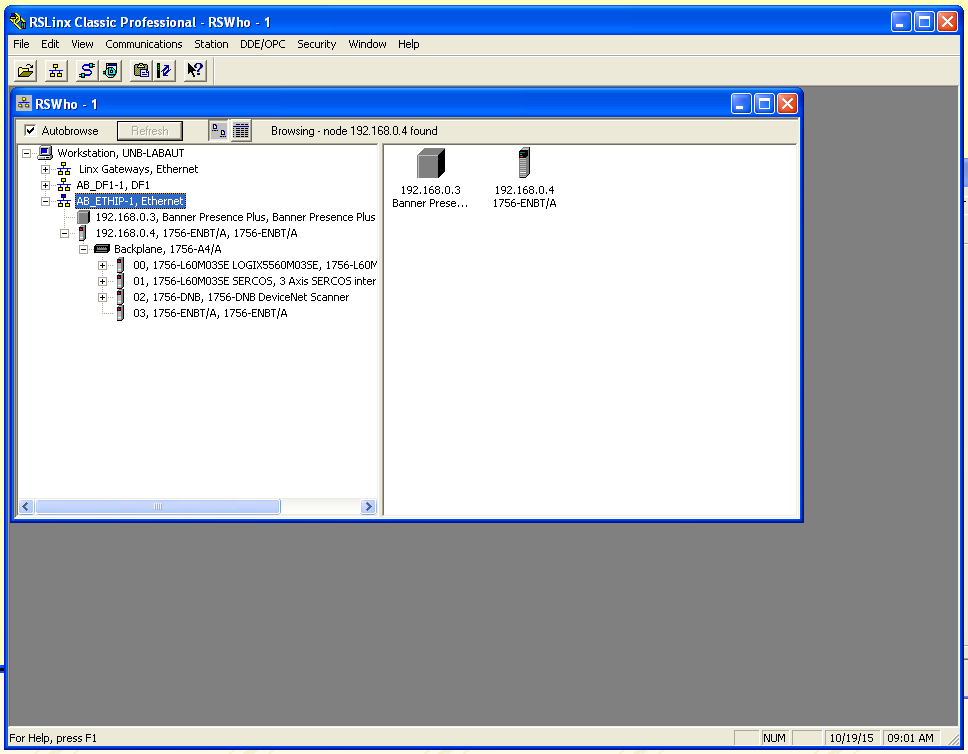
\includegraphics[width=\linewidth]{figs/resultados/camera/cameralinx}
\caption{RSLinx com câmera reconhecida \label{linxcamera}}
\end{figure}

\subsection{Calibração}

A câmera permite fazer medidas de distâncias em \textit{pixels}. De forma a se converter essa distância para milímetros, uma barra de alumínio com marcas e tamanho conhecido é utilizada. É importante primeiro calibrar o sistema, para se saber se há deformação de pixels significante ao longo da distância de interesse, nomeadamente o tamanho da barra de alumínio sendo utilizada, cerca de $532$mm. No PresencePlus P4 GEO 1.3, um programa é feito, com imagem de referência conforme Figura \ref{cameracalibracao}, que usa várias ferramentas de detecção de borda (ferramenta \texttt{Locate}) para identificar as posições de cada uma das marcas pretas da barra. Seis marcas foram feitas e a Tabela \ref{relacoesmmpx} apresenta os resultados para cada seção. A distância entre duas marcas é de 10cm, com exceção da distância entre P0 e PEND que é o comprimento total da barra.

\begin{figure}[!ht]
\centering
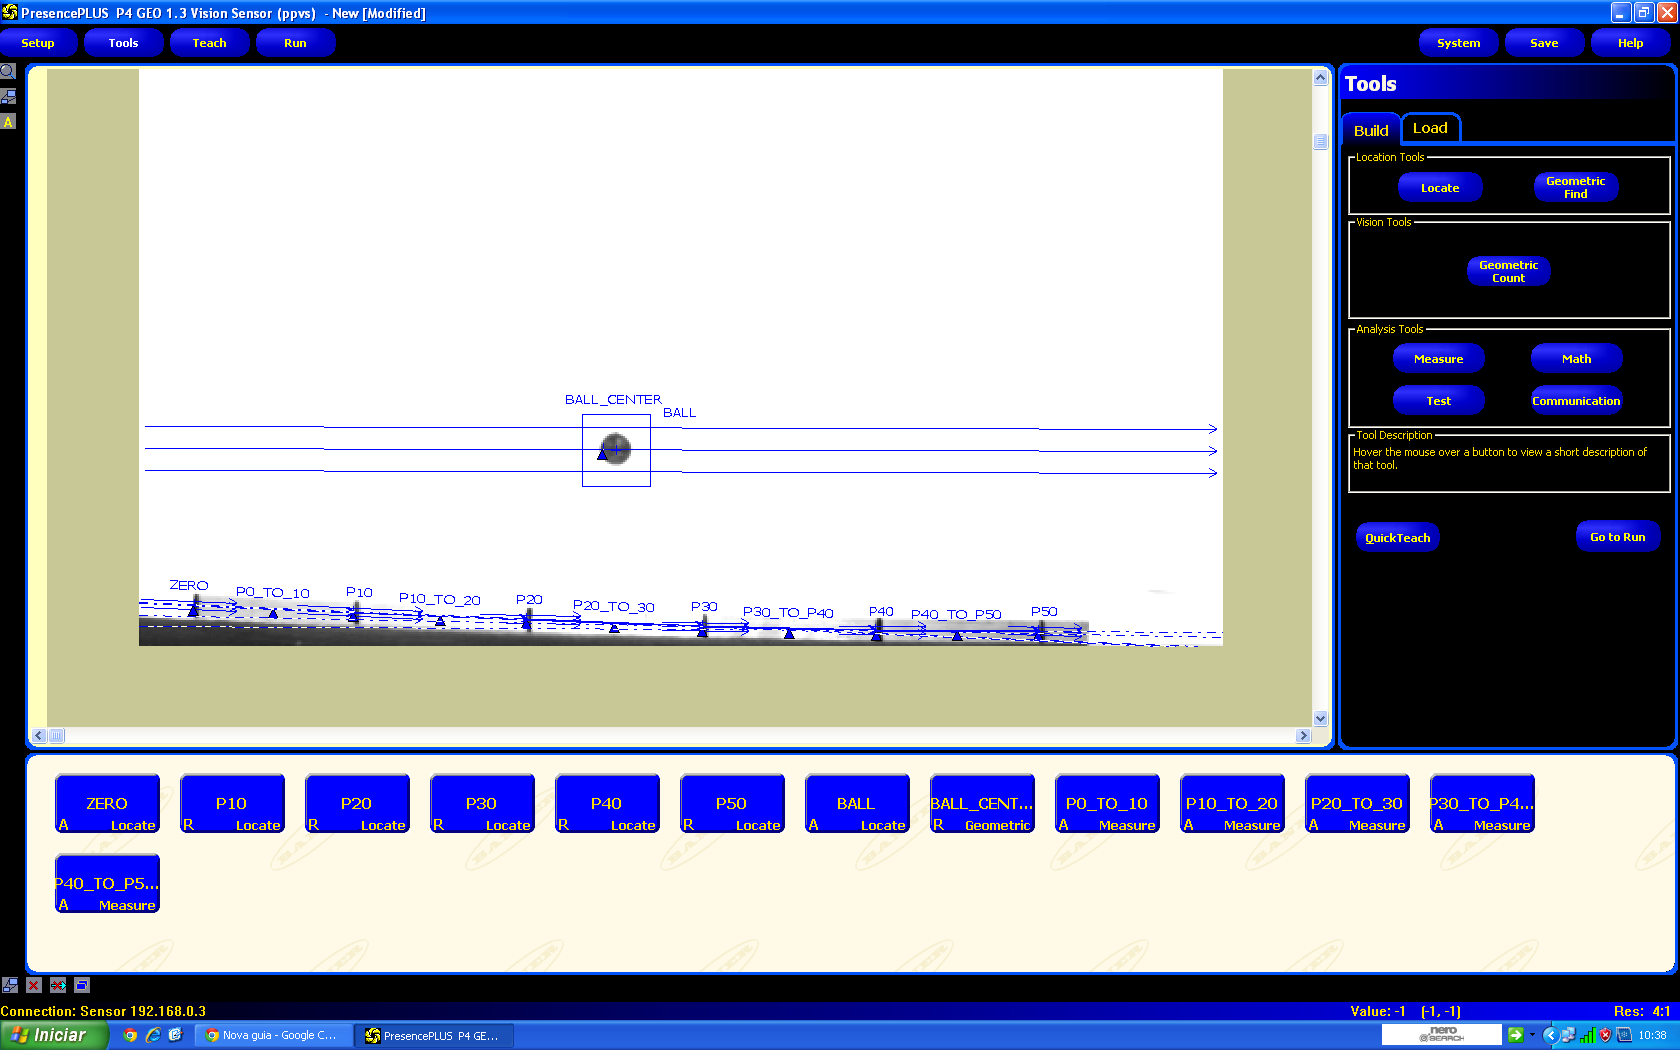
\includegraphics[width=0.9\linewidth]{figs/resultados/camera/programa}
\caption{Programa PresencePLUS para calibração da câmera \label{cameracalibracao}}
\end{figure}

\begin{table}[!ht]
\centering
\caption{Relações mm/px para diferentes seções da barra de alumínio \label{relacoesmmpx}}
	\begin{tabular}{|c|c|c|c|}
	\hline
		Seção 1 & Seção 2 & Distância (px) & mm/px\\ \hline
		P0 & P10 & 160 & 0.625\\ \hline
		P10 & P20 & 173 & 0.578\\ \hline
		P20 & P30 & 176 & 0.568\\ \hline
		P30 & P40 & 173 & 0.578\\ \hline
		P40 & P50 & 163 & 0.613\\ \hline
		P0 & PEND & 893 & 0.596\\ \hline
	\end{tabular}
\end{table}

O maior desvio da quantidade de milímetros por \textit{pixel} das seções em relação à da barra inteira é de aproximadamente 4.93\%. Há algumas imprecisões na maneira como os traços foram desenhados e é possível que o erro seja menor.

\subsection{Programação}
A programação da câmera inicia obtendo uma imagem de referência e adicionando-se ferramentas de detecção de pontos de interesse, como mostra a Figura \ref{cameracalibracao}. A ferramenta \texttt{Locate} é responsável por detectar as bordas da bolinha, e a ferramenta \texttt{Geometric} detecta o centro da mesma. Também é possível adicionar ferramentas que fazem operações matemáticas (ferramenta \texttt{Math}), executam medições (ferramenta \texttt{Measure}), assim como as que enviam dados pela rede (ferramenta \texttt{Communication}), o que é essencial para comunicar com o CLP.

\section{Calibração do Servomotor\label{calibracaoServomotorSecao}}

O RSLogix tem o bloco \texttt{MAJ} \textendash{} \textit{Motion Axis Jog} \textendash{} que permite alterar a velocidade do motor enquanto ele se movimenta. No entanto, o bloco espera que a entrada seja do tipo $[\mathrm{u}/\mathrm{s}$ ao invés de alguma unidade no SI tal como $[\mathrm{mm}/\mathrm{s}]$. Devido a isso, foi necessária uma calibração do sistema. Nela, anotou-se a posição inicial $x_0$ e a posição final $x_f$, ambas em milímetros, e definia-se um tempo $\Delta t$ no qual o carrinho se movimentaria a uma velocidade $v$ em $[\mathrm{u}/\mathrm{s}]$. Daí, calculava-se a velocidade em $[\mathrm{mm}/\mathrm{s}]$ com esses dados e tirou a média de alguns ensaios para se obter o valor de uma unidade, que é aproximadamente $71.32\mathrm{mm}$. Os dados de calibração estão na Tabela \ref{calibracaoServomotor}.

\begin{table}[!ht]
\centering
\caption{Dados de calibração do servomotor, média obtida é de 71.32 mm/unidade\label{calibracaoServomotor}}
\begin{tabular}{|c|c|c|c|c|c|}
\hline
	$x_0$ - [mm] & $x_f$ - [mm] & $\Delta t$ - [s] & Velocidade - [u/s] & Velocidade - [mm/s] & mm/u\\ \hline
2 &	71.8  &	2   &	0.5 &	34.9   & 	69.8\\ \hline
6 & 76.1  &	2   &	0.5 &	35.05  &	70.1\\ \hline
6 &	188	  &  5   &	0.5	&   36.4   &	72.8\\ \hline
6 &	185   &	2.5 &	1	& 	71.6   &	71.6\\ \hline
6 &	77    &	10  &	0.1	&   7.1    &	71\\ \hline
6 &	296.5 &	20	&   0.2 & 	14.525 &	72.625\\ \hline\end{tabular}
\end{table}

\section{Modelo no Espaço de Estados}

A partir da teoria apresentada na subseção \ref{reducaoModal}, desenvolveram-se algumas rotinas em linguagem Julia \cite{julia} para obter as matrizes reduzidas. A ordem da matriz de saída é um parâmetro. A Seção \ref{reducaoModalPrograma} dos anexos apresenta o código completo.

As matrizes dos modelo reduzidos são apresentadas nas Equações \ref{modeloReduzidoSemEpsilon} e \ref{modeloReduzidoComEpsilon}. Antes da compensação do atraso, o sistema é representado pela Equação \ref{modeloEspacoDeEstadosSemAtraso}. Quando se analisa a resposta ao degrau em malha aberta para este caso, Figura \ref{modeloMalhaAberta}, nota-se que o atraso é cerca de 0.3s. Para ser preciso, $\epsilon = 0.313$s. Utilizando esse atraso, a transferência direta se tornaria aproximadamente zero. No entanto, esses modelos no espaço contínuo serão discretizados com período $T_s = 0.1$s. Daí, o $\epsilon$ mais próximo é 0.3s. Apesar de próximo, esse atraso não reduz muito a transferência direta, como se pode observar a diferença entre $D_R$, Equação \ref{modeloReduzidoSemEpsilon}, e $D_D$, Equação \ref{modeloReduzidoComEpsilon}.

\begin{align}
\left.\begin{array}{ll}
	\mathbf{A_R} &= \left[\begin{array}{cccc}
		-0.0881  & -3.8389 &         0 &         0\\
    3.8389 &   -0.0881 &         0 &         0\\
         0 &         0 &   -0.1061 &  -10.8145\\
         0 &        0 &   10.8145 &   -0.1061\\
	\end{array}\right]\\
	\mathbf{B_R} &= 10^3\left[0.3313,\;
    0.0066,\;
    1.3549,\;
    0.0163\right]^{\mathrm{T}}\\
	\mathbf{C_R} &= \left[-0.0003,\;0.0148,\;0.0001,\;-0.0029\right]\\
	D_R &= -0.0906
\end{array}\right\} \label{modeloReduzidoSemEpsilon}
\end{align}

\begin{align}
\left.\begin{array}{ll}
	\mathbf{B_D} &= 10^3\left[0.1255,\;
    0.2974,\;
   -1.3039,\;
   -0.1504\right]^{\mathrm{T}}\\
	D_D &= -0.0685
\end{array}\right\} \label{modeloReduzidoComEpsilon}
\end{align}

\begin{align}
	\left.\begin{array}{ll}
		\mathbf{\dot{z}} &= \mathbf{A_R}\mathbf{z} + \mathbf{B_R}u(t)\\
		y &= \mathbf{C_R}\mathbf{z} + \mathbf{D_R}u(t)
	\end{array}\right\}\label{modeloEspacoDeEstadosSemAtraso}
\end{align}

\begin{align}
	\left.\begin{array}{ll}
		\mathbf{\dot{z}} &= \mathbf{A_R}\mathbf{z} + \mathbf{B_D}u(t-\epsilon)\\
		y &= \mathbf{C_R}\mathbf{z} + \mathbf{D_D}u(t-\epsilon)
	\end{array}\right\}\label{modeloEEComAtraso}
\end{align}

\begin{figure}[!ht]
\centering
\caption{Resposta ao degrau para modelos reduzidos com atraso e sem atraso\label{modeloMalhaAberta}}
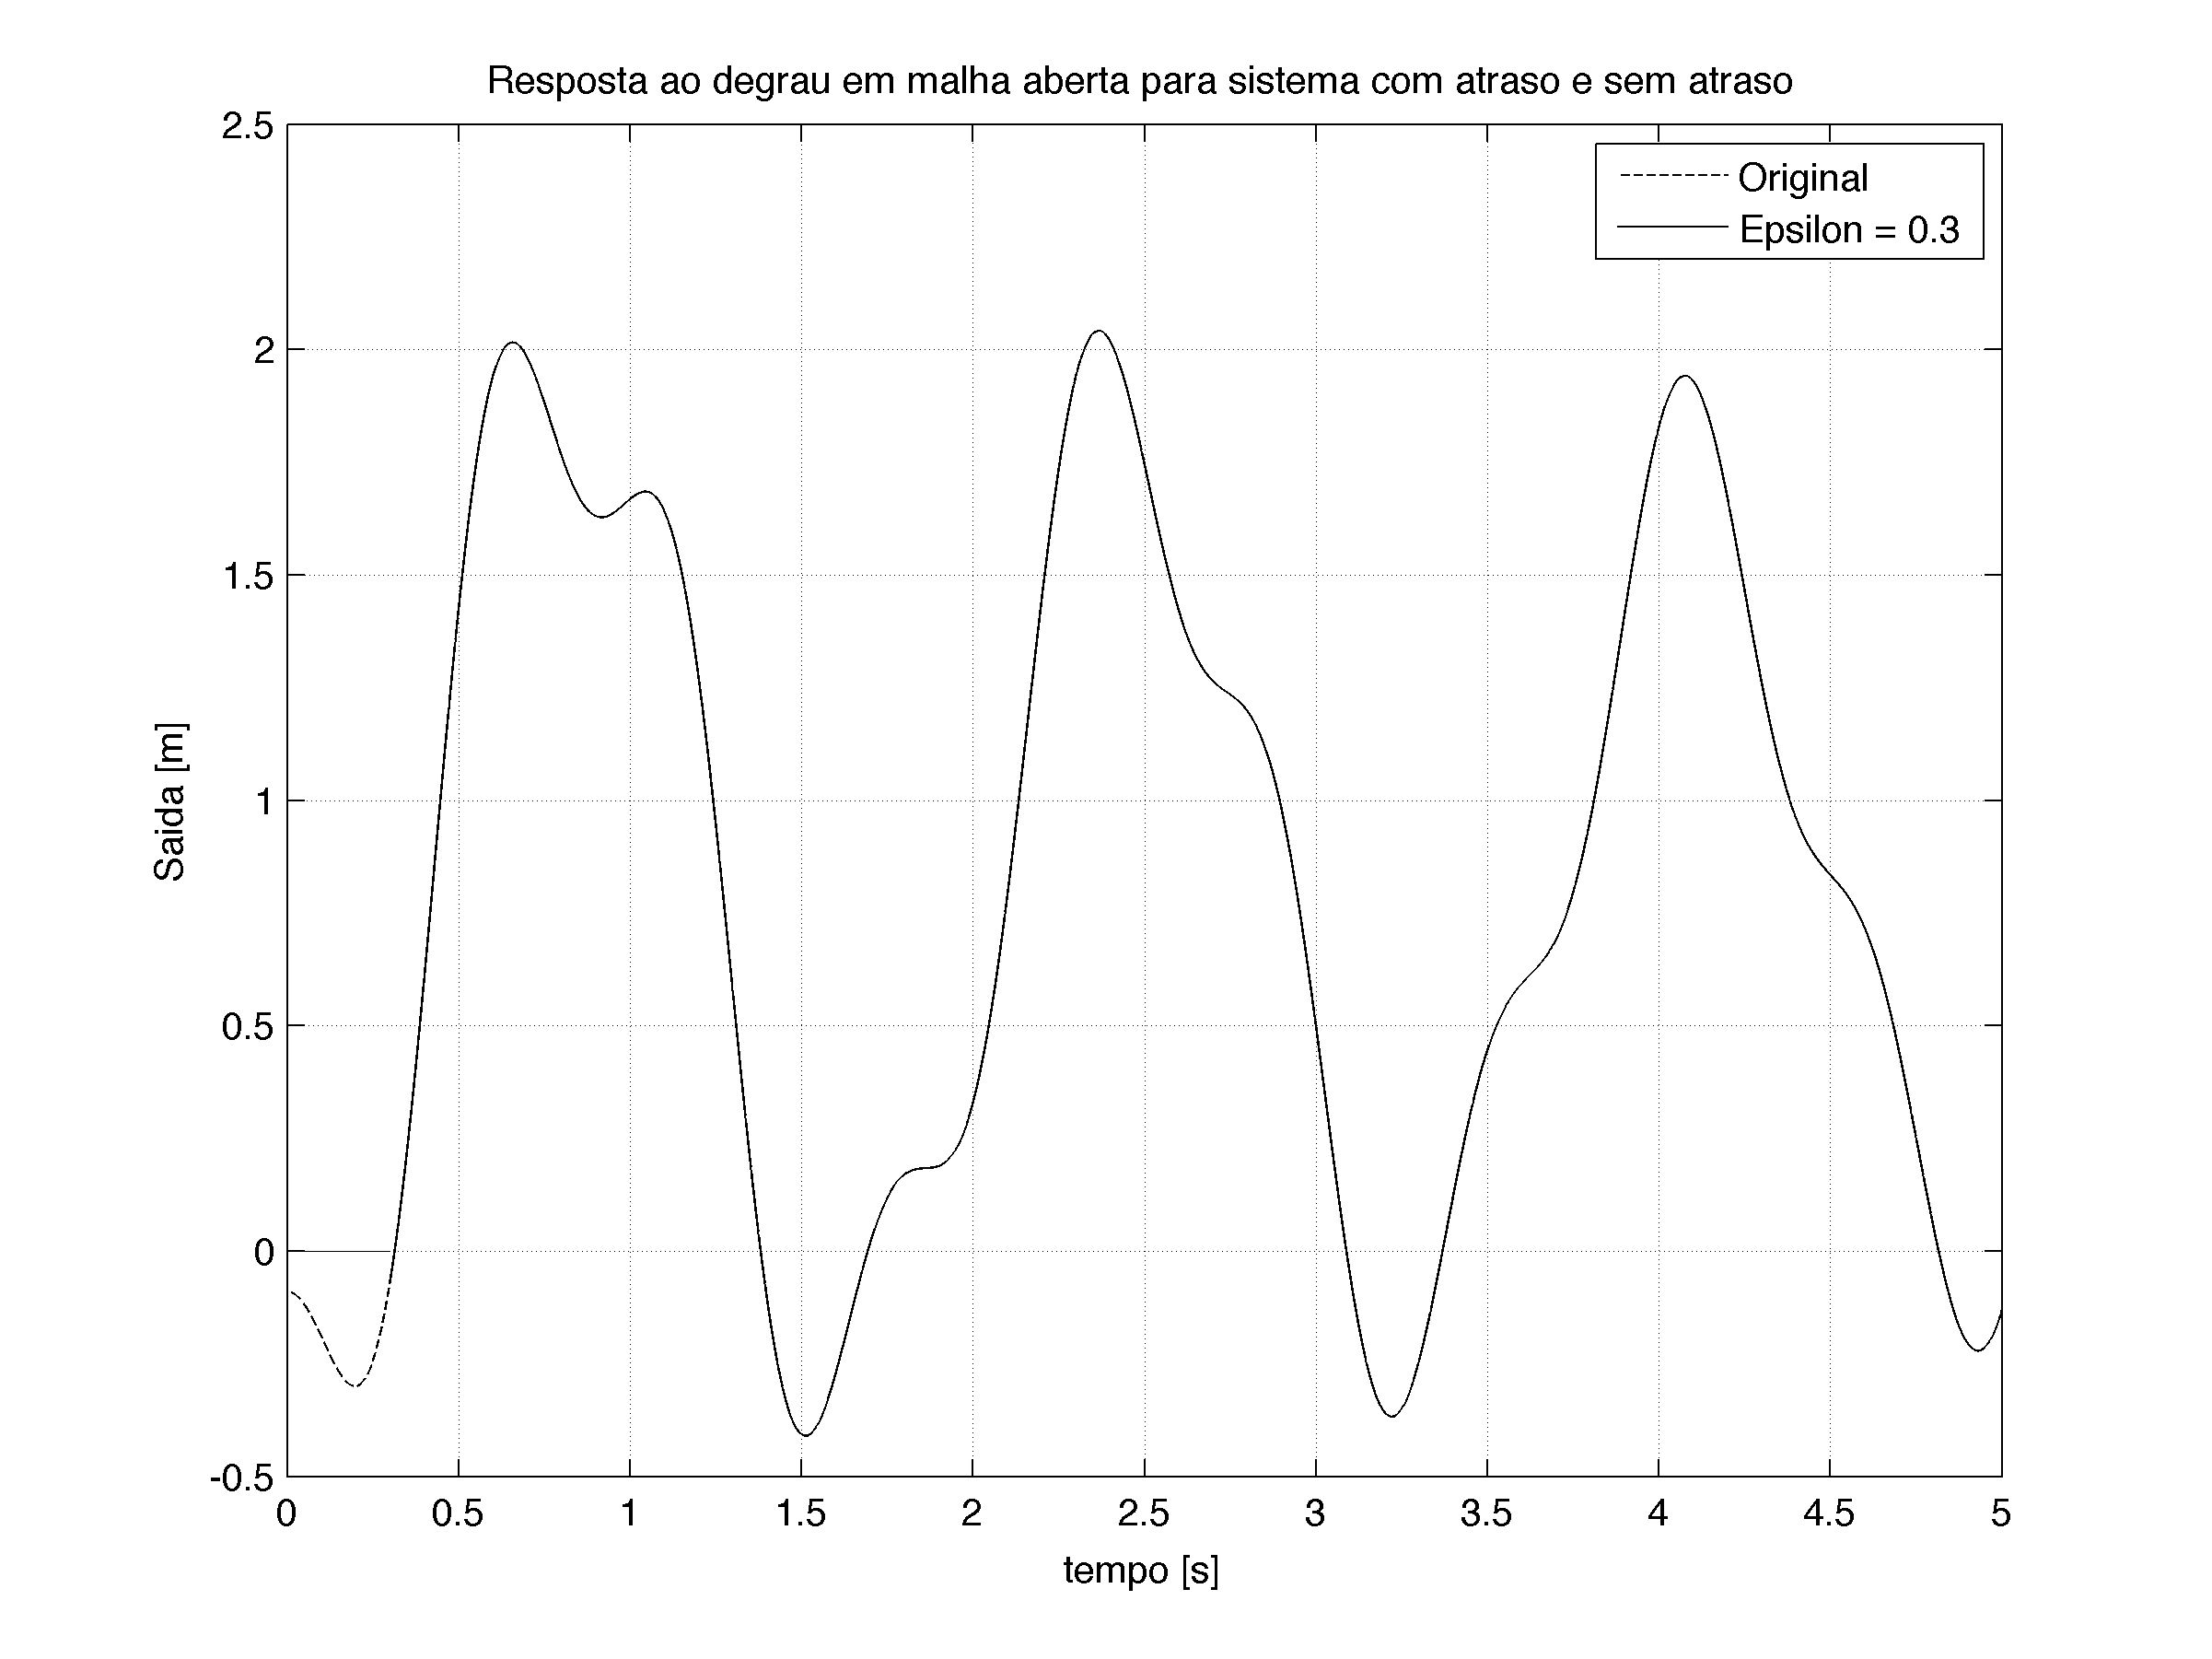
\includegraphics[width=0.8\linewidth]{figs/resultados/modelo/respostaMalhaAberta}
\end{figure}

 O sistema em malha aberta oscila muito, mas é estável. Observa-se que a resposta decai conforme o tempo passa, conforme Figura \ref{modeloMalhaAberta25s}. O objetivo do controle é reduzir ao máximo essas oscilações, tendo uma trajetória o mais suave possível de um ponto inicial a um ponto final. Para ter uma melhor ideia quantitativa, calculam-se os autovalores da matriz $\mathbf{A_R}$, resultando em \begin{align}
 	\mathrm{eig}\left(\mathbf{A_R}\right) &= \left[-0.0881 \pm 3.8389j,\;
  -0.1061 \pm 10.8145j\right].
 \end{align}

\begin{figure}[!ht]
\centering
\caption{Resposta ao degrau para modelos reduzidos com atraso e sem atraso, 25 segundos\label{modeloMalhaAberta25s}}
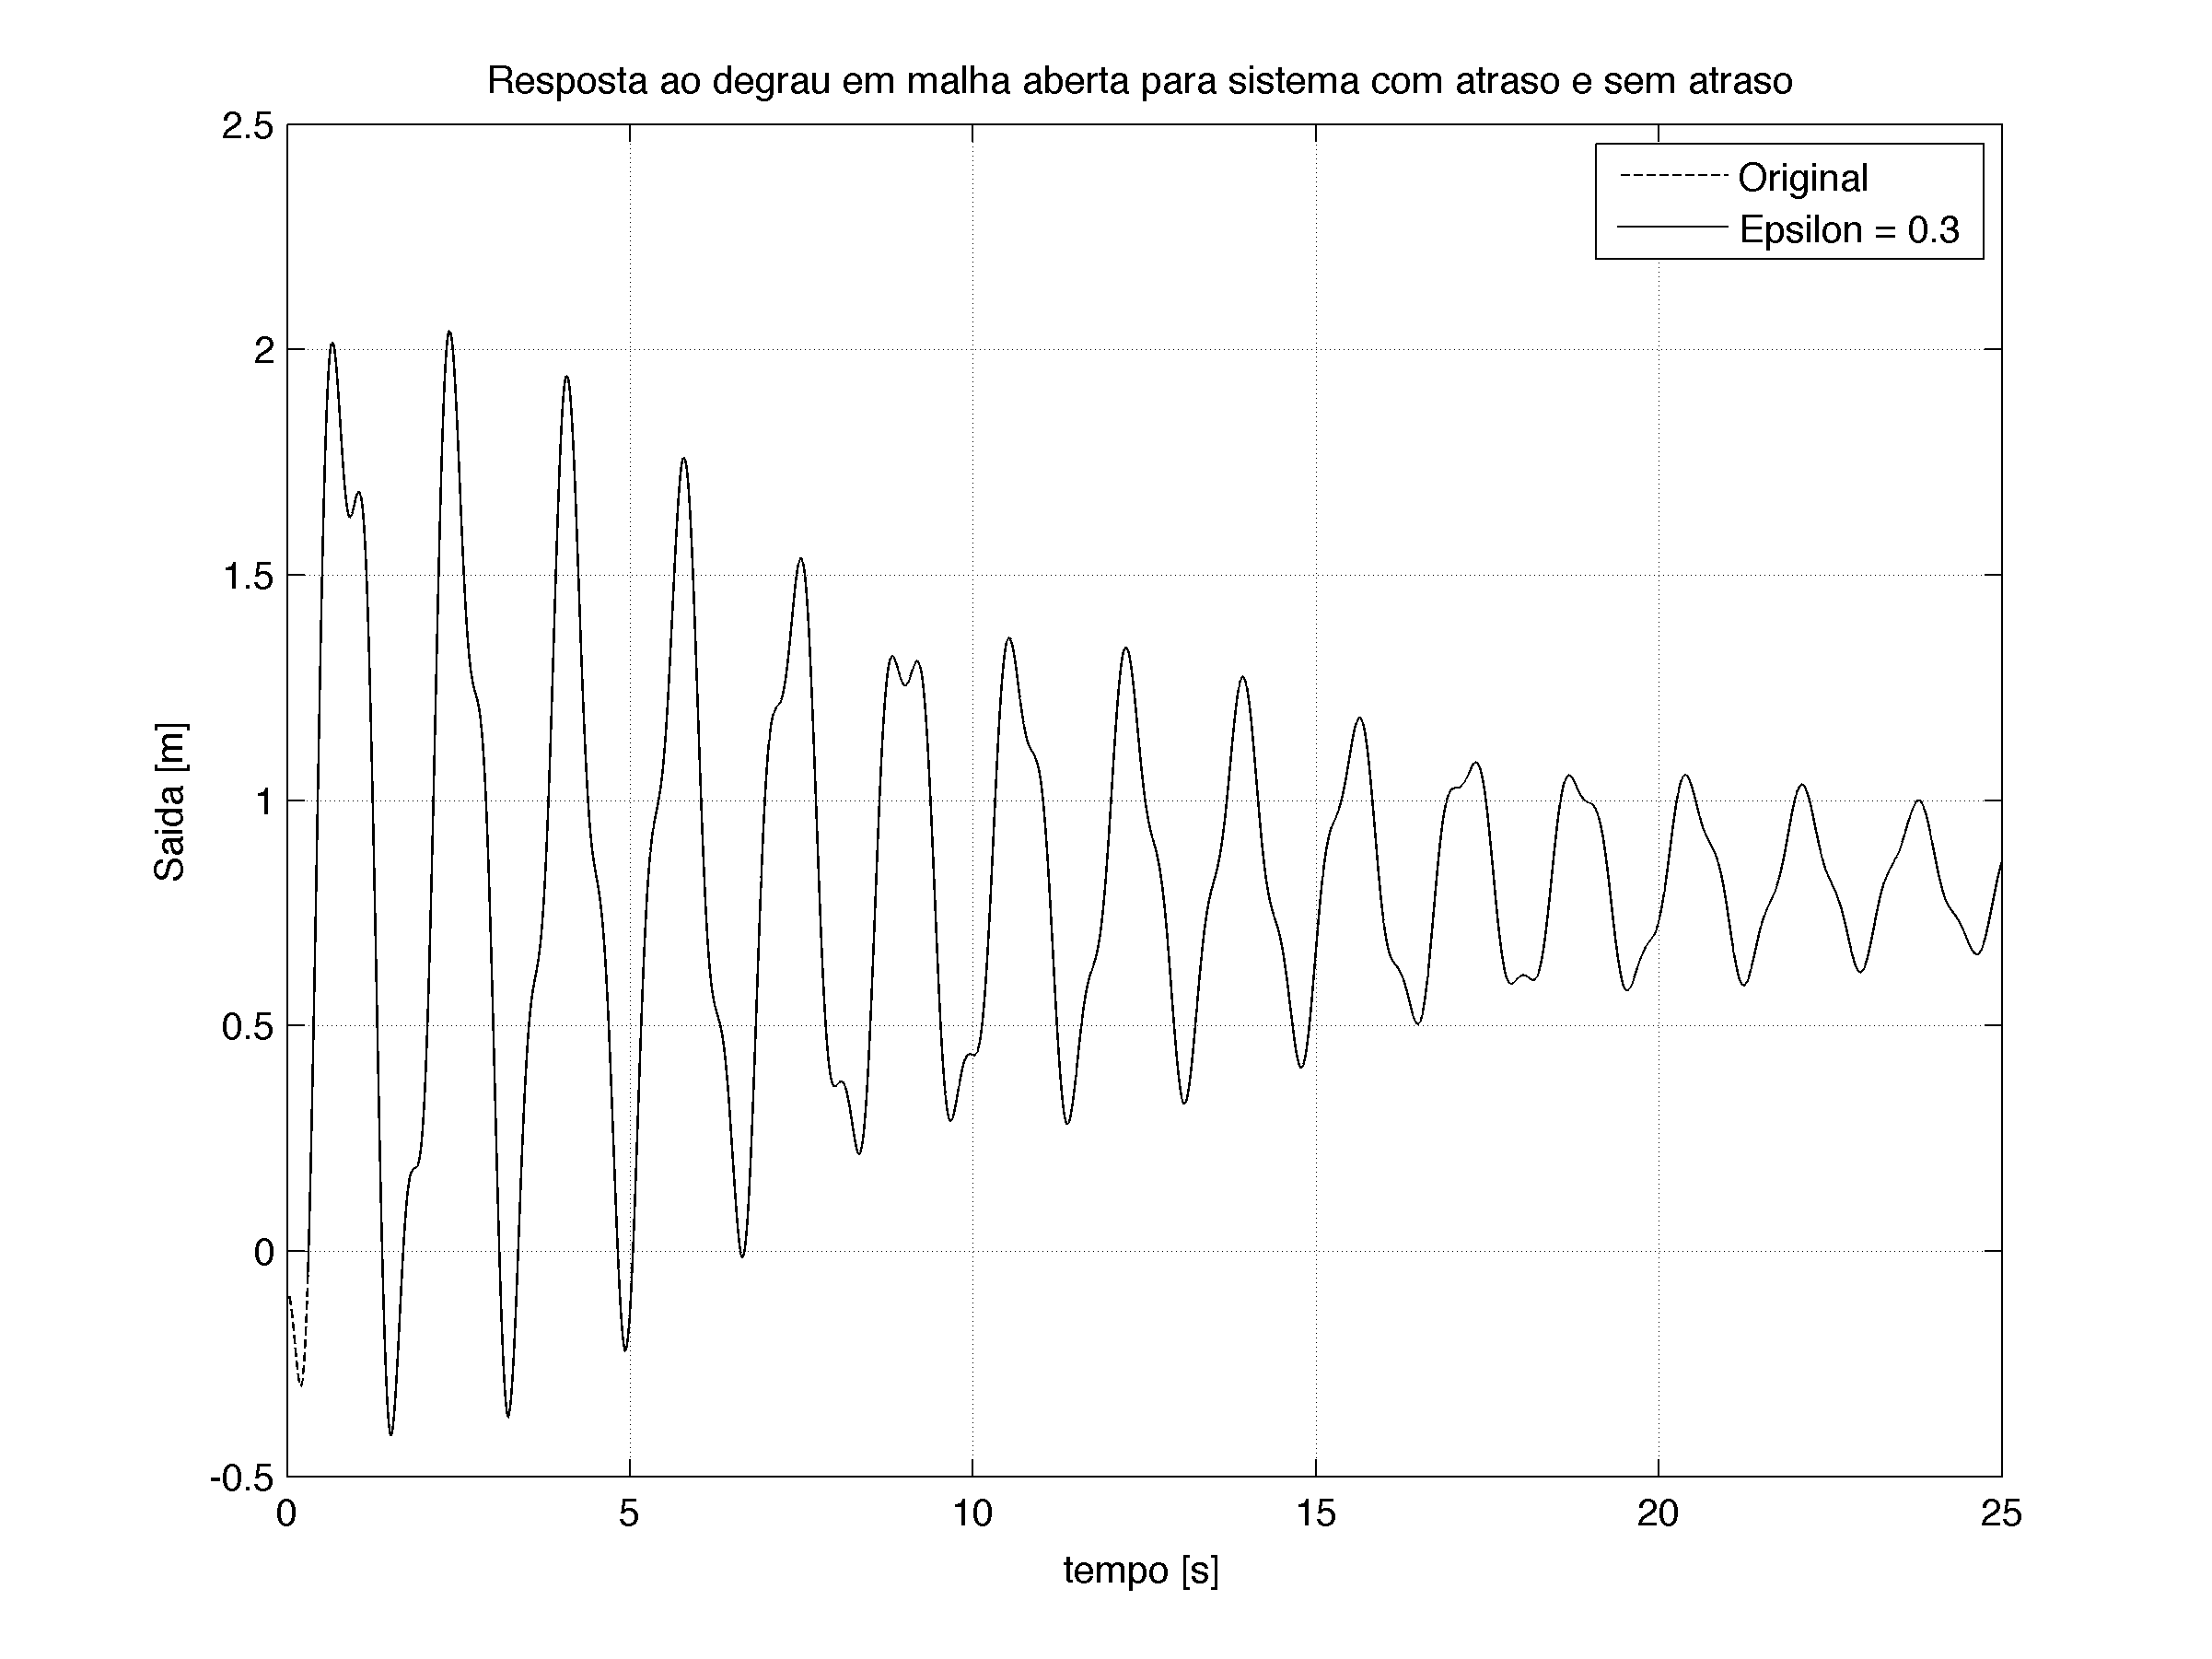
\includegraphics[width=0.8\linewidth]{figs/resultados/modelo/respostaMalhaAberta25s}
\end{figure}

\subsection{Discretização}
 O controle será feito conforme a Seção \ref{controle}, mas primeiro deve-se discretizar o sistema. A função \texttt{c2d} \cite{c2d} do MATLAB é utilizada, resultando nas matrizes \begin{align}
 \begin{array}{ll}
 	\mathbf{A} &= \left[\begin{array}{cccc}
	0.9191&   -0.3712&         0&         0\\
    0.3712&    0.9191&         0&         0\\
         0&         0&    0.4651&   -0.8733\\
         0&         0&    0.8733&    0.4651\\
 \end{array}\right],\\
 	\mathbf{B} &= \left[6.5818,\;
   31.2517,\;
  -98.5991,\;
  -75.6695\right]^{\mathrm{T}},\\
   \mathbf{C} &= \left[-0.0003,\;0.0148,\;0.0001,\;-0.0029\right],\\
   D &= -0.0685.
 \end{array}
 \end{align}
 
 Os polos de $\mathbf{A}$ são $0.9191 \pm 0.3712j$ e $
   0.4651 \pm 0.8733j$. Como esses polos estão dentro do círculo unitário, o sistema continua estável, apesar de manter as oscilações, como se nota pelo fato dos polos terem parte imaginária. Note que as matrizes $\mathbf{C}$ e $D$ são iguais a $\mathbf{C_R}$ e $D_D$ do sistema contínuo, respectivamente, conforme Equações \ref{modeloReduzidoSemEpsilon} e \ref{modeloReduzidoComEpsilon}.
 
\subsection{Controle}

 A parte mais difícil do controle é a escolha dos polos. Algumas simulações foram realizadas e observava-se se o sistema era estável e se oscilava muito. O projeto final considerou 5 polos $\left[0.6,\;0.6,\;0.6,\;0.5\pm 0.4j\right]$. O primeiro polo se deve ao integrador que foi adicionado ao sistema. Os ganhos para esse caso são dados por \begin{align}
 	\mathbf{K_p} &= \left[0.0080,\;0.0096,\;-0.0046,\;-0.0004\right],\\
 	K_i &= 0.1953.
 \end{align}
 
 O código para calcular os ganhos está disponível na Seção \ref{projetoControlador}.

\section{Simulação}

\begin{figure}[!ht]
\centering
\caption{Esquema principal para simulação em Simulink\label{topModel}}
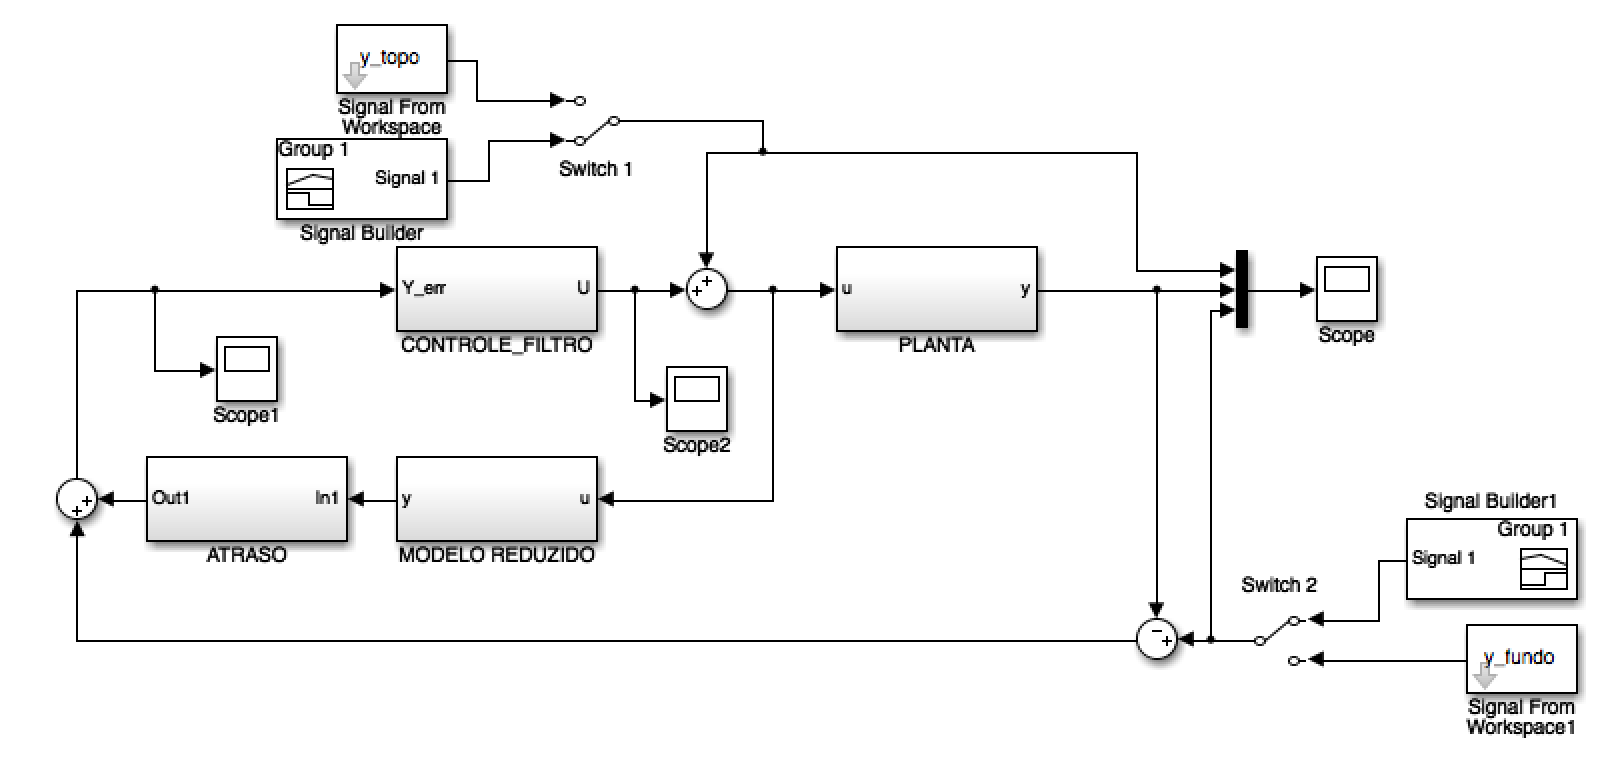
\includegraphics[width=0.9\linewidth]{figs/resultados/simulink/top}
\end{figure}

\begin{figure}[!ht]
\centering
\caption{Bloco de Atraso -- saída é o valor antecipado menos um valor antigo\label{blocoAtraso}}
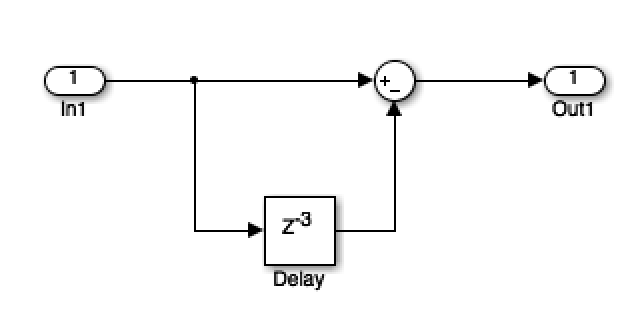
\includegraphics[width=0.5\linewidth]{figs/resultados/simulink/atraso}
\end{figure}

\begin{figure}[!ht]
\centering
\caption{Modelo reduzido -- não utiliza atraso, utilizado para predizer a saída\label{blocoModeloReduzido}}
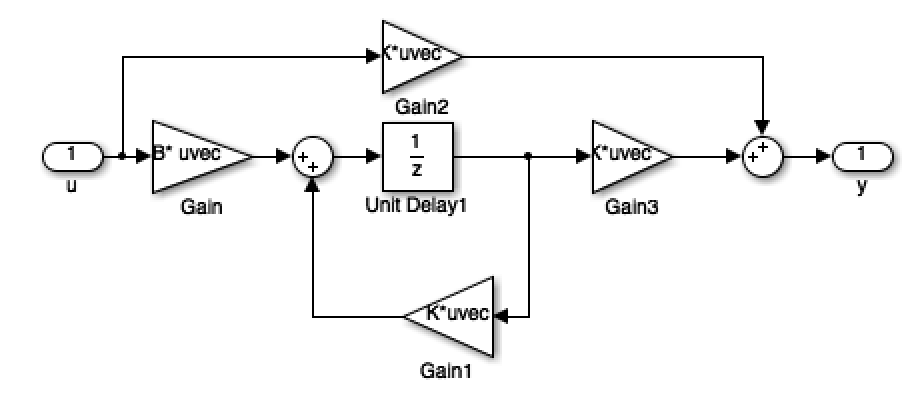
\includegraphics[width=0.6\linewidth]{figs/resultados/simulink/modeloReduzido}
\end{figure}

\begin{figure}[!ht]
\centering
\caption{Bloco de controle com filtro de Kalman\label{blocoControle}}
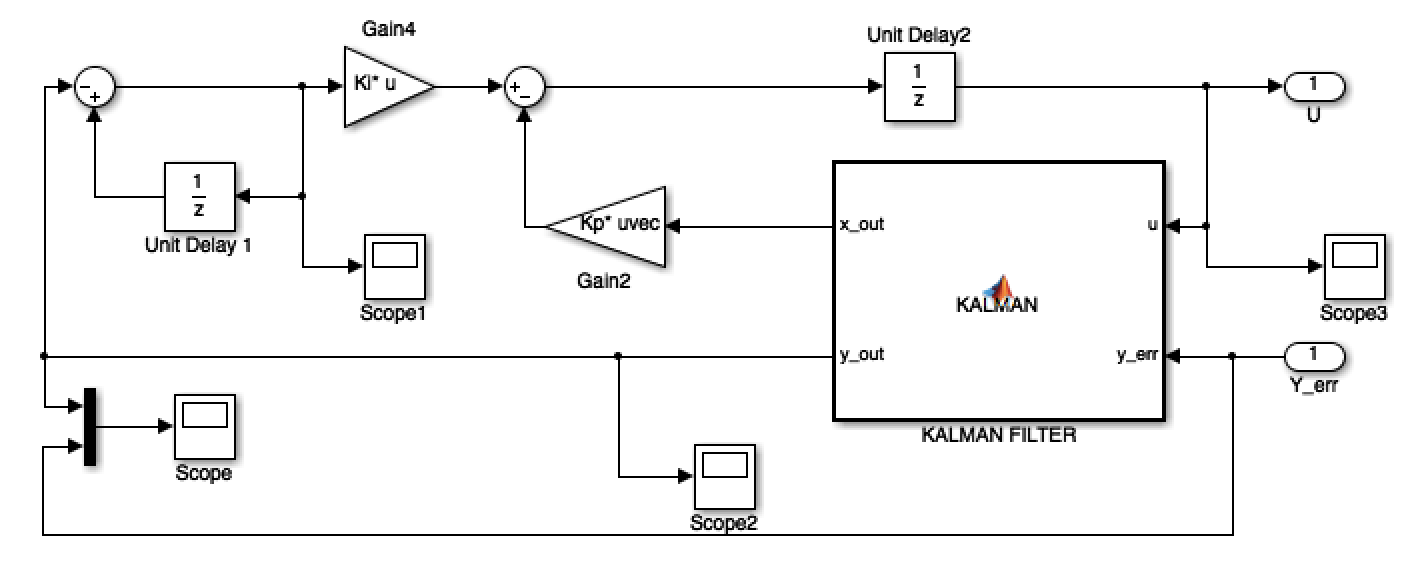
\includegraphics[width=0.9\linewidth]{figs/resultados/simulink/controle}
\end{figure}



\section{Malha aberta}

O planejamento de trajetória em malha aberta e malha fechada para o \textit{riser} que está sendo utilizado neste trabalho foi desenvolvido por Fabrício et al \cite{fabricioIFAC}, conforme mencionado anteriormente. Um programa em MATLAB foi escrito e gerou trajetórias de excursão pré-definida. Rédytton \cite{redytton} testou o sistema para uma excursão de cerca de 1m, que é maior que o tamanho do barbante ($82\mathrm{cm}$) conforme apresentado na Tabela \ref{escalaLaboratorial}. No entanto, seu trabalho não utilizou uma massa de isopor na ponta, daí existirá uma diferença entre os resultados. Observe que, em malha aberta, deixou-se o ar condicionado da sala desligado, pois isto seria uma perturbação.

\subsection{Excursão de 30cm}
O primeiro teste em malha aberta testou a trajetória de posição da Figura \ref{DeslocamentoT1}. Conforme Rédytton \cite{redytton} mencionou em seu trabalho, utilizar os módulos de posição é mais lento do que utilizar módulos de velocidade para seguir essa trajetória. Desta forma, optou-se por usar diferenças finitas para derivar essa trajetória, resultando na Figura \ref{VelocidadeT1}. 

\begin{figure}[!htb]
    \centering
    \begin{minipage}{.45\textwidth}
        \centering
        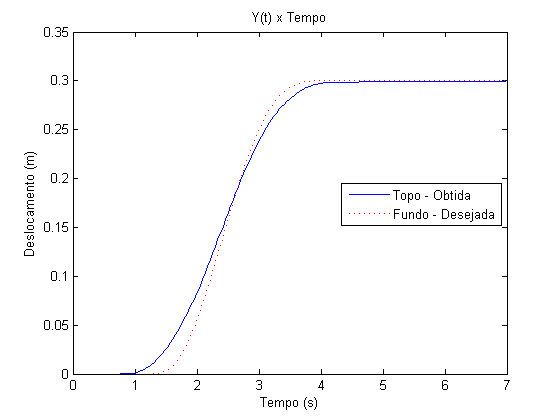
\includegraphics[width=1\linewidth]{figs/resultados/malha_aberta_1/DeslocamentoT1}
        \caption{Referência de Posição para Excursão de 30cm}
        \label{DeslocamentoT1}
    \end{minipage}%
    \hspace{0.1cm}
    \begin{minipage}{0.45\textwidth}
        \centering
        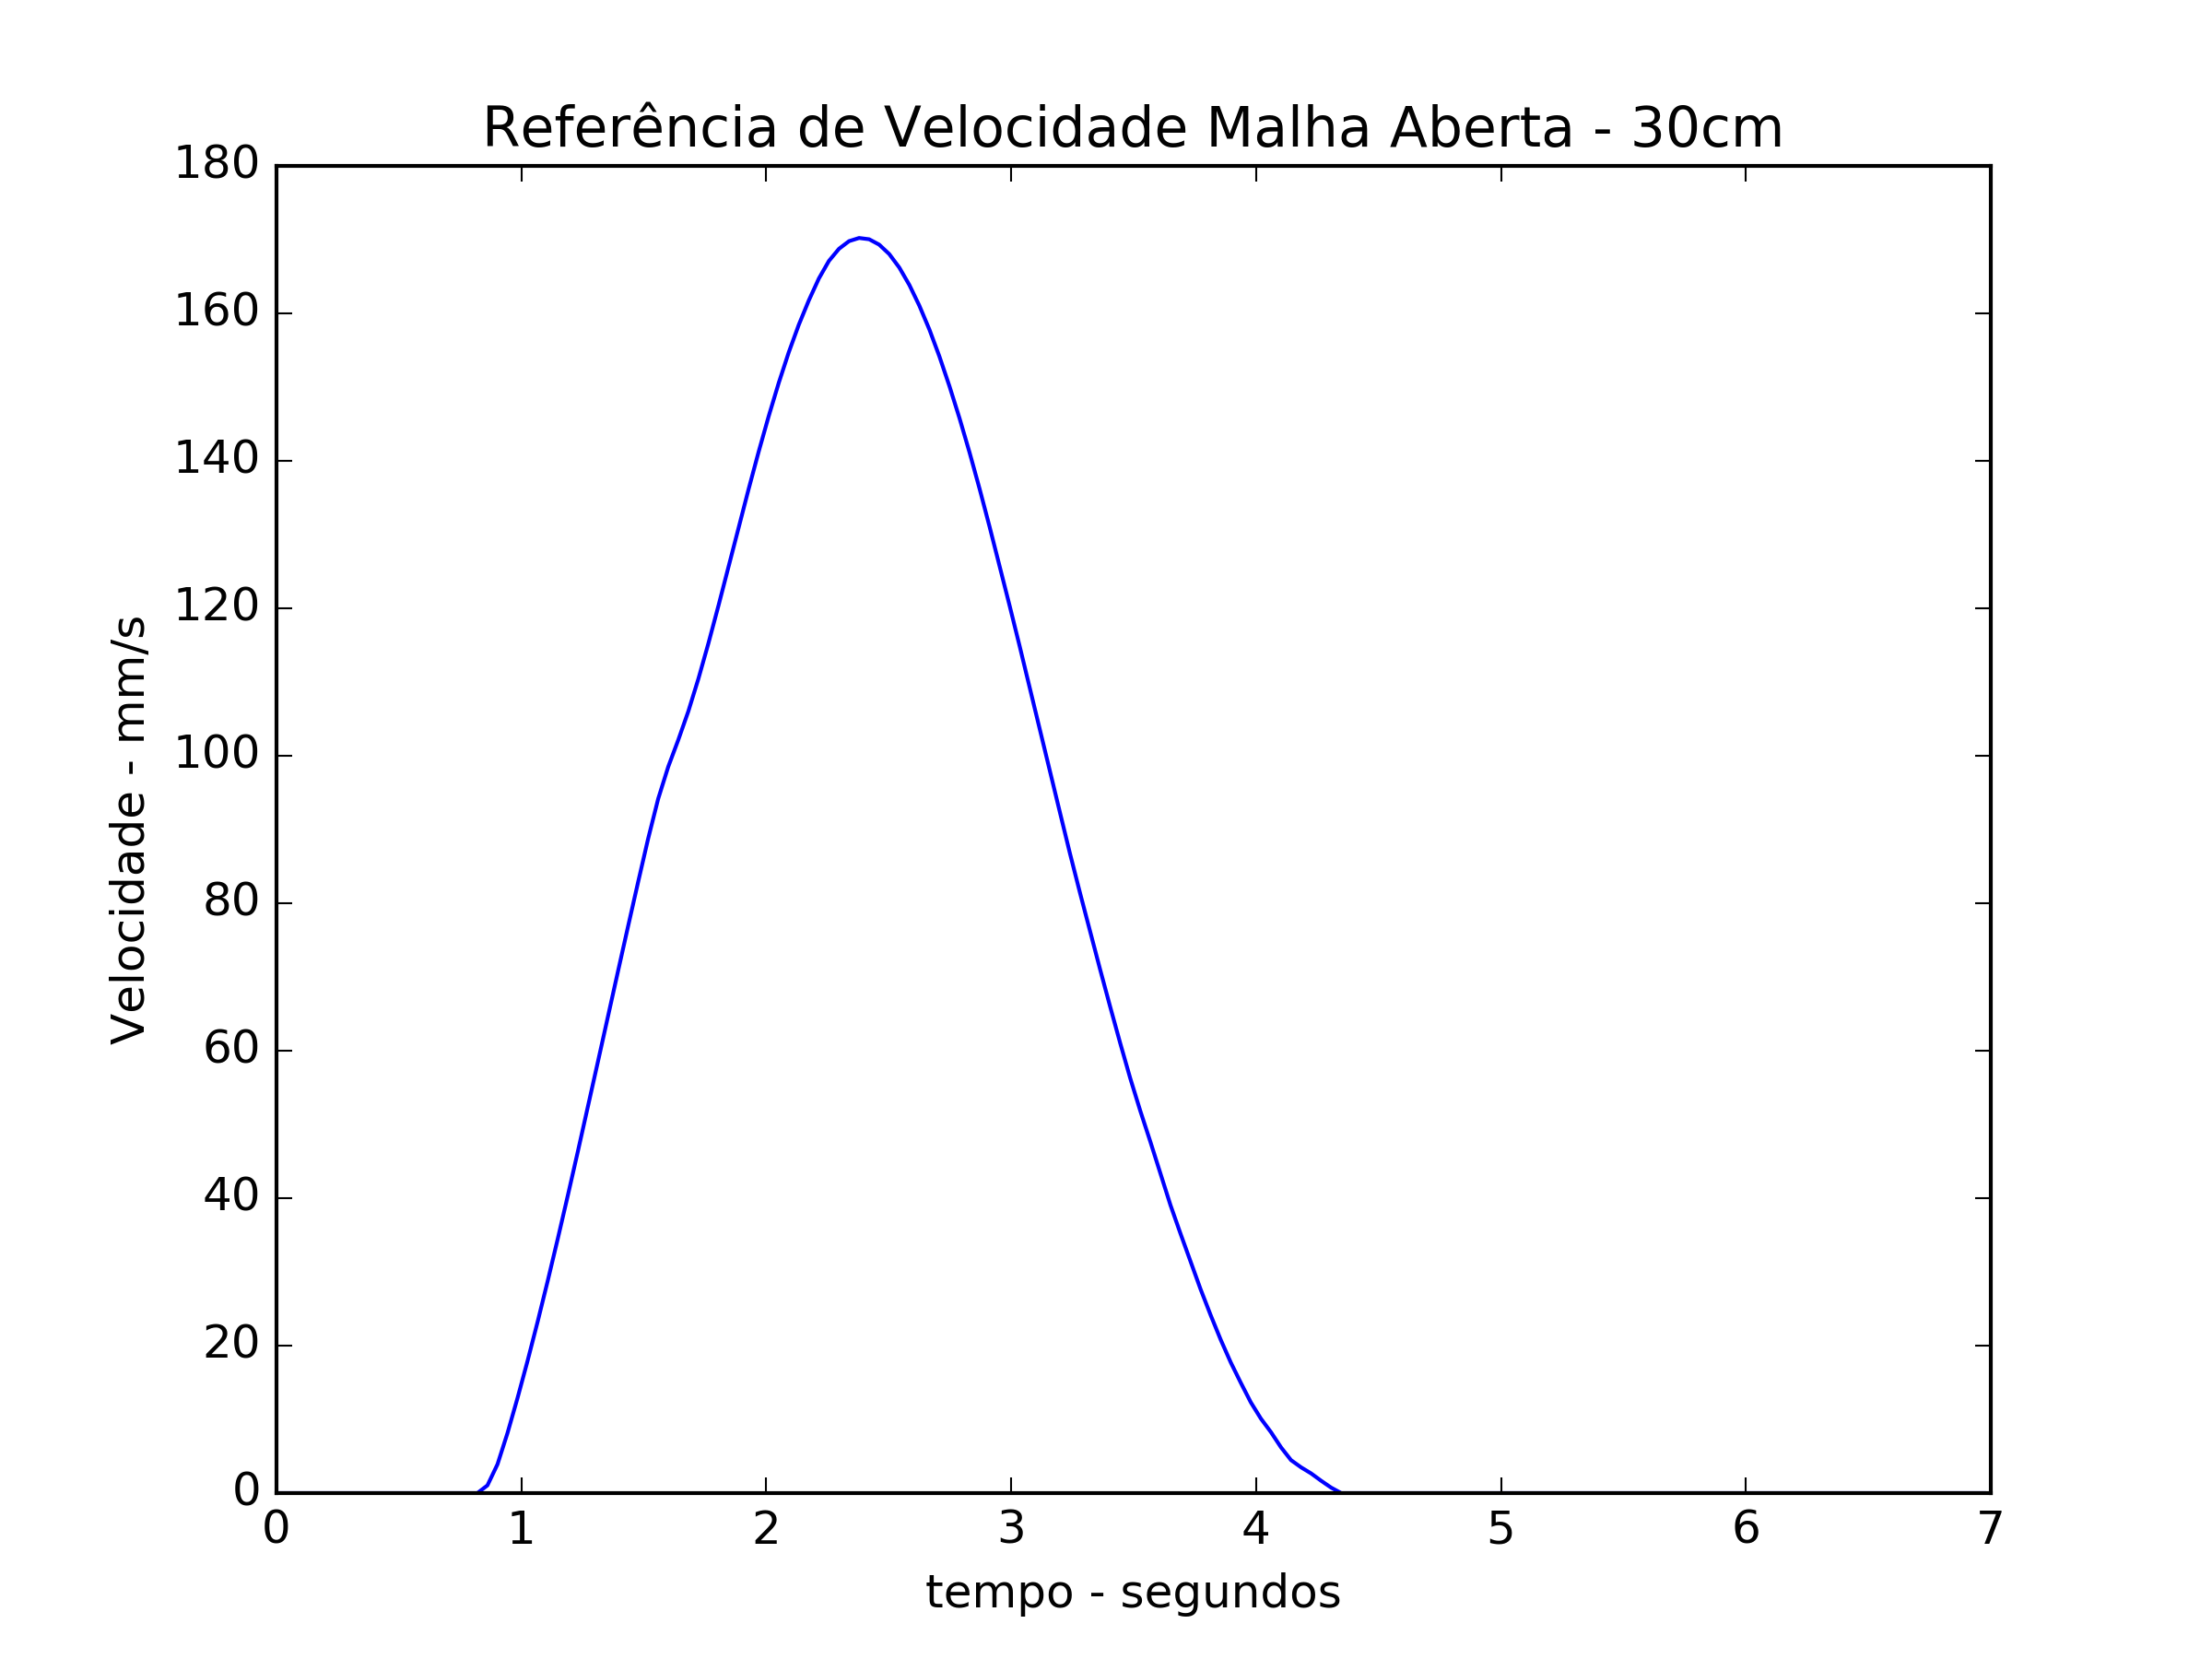
\includegraphics[width=1\linewidth]{figs/resultados/malha_aberta_1/VelocidadeT1}
        \caption{Referência de Velocidade para Excursão de 30cm}
        \label{VelocidadeT1}
    \end{minipage}
\end{figure}

Com um período de cerca de 41ms, uma tarefa eventual executava no CLP, aplicando um certo valor de velocidade ao carrinho. A câmera leu os valores de posição cada vez que a tarefa iniciava e o software RSLogix desenhou os dados, que podem ser observados na Figura \ref{trajetoriaObtidaModelada}. Observa-se que a posição evolui de forma bem suave. Para se realizar uma comparação, calculou-se o tempo que o carrinho se move na trajetória ($\Delta t$, tempo no qual a velocidade não é nula) e calculou-se $\overline{v} = \frac{\Delta x}{\Delta t}$. No caso presente, $\Delta x = 30\mathrm{cm}$ e $\Delta t \approx 3\mathrm{s}$ (veja Figura \ref{VelocidadeT1}), resultando em $\overline{v} = 100\mathrm{mm}/\mathrm{s}$. A Figura \ref{trajetoriaObtidaVConstante} apresenta esses resultados e observa-se várias oscilações quando o carrinho para, diferente do caso anterior.

Vídeos foram criados para cada um destes casos e estão disponíveis no YouTube{\sffamily\textregistered\textcopyright}, tanto para a trajetória modelada\footnote{Controle Malha Aberta Modelado, 30cm - \url{https://youtu.be/lKajz6LyauE}. Acesso em 29/11/2015.} quanto para a trajetória com velocidade constante\footnote{Controle Malha Aberta a Velocidade Constante, 30cm - \url{https://youtu.be/tB0TsmBcfVg}. Acesso em 29/11/2015.}.

\begin{figure}[!htb]
    \centering
    \begin{minipage}{.45\textwidth}
        \centering
        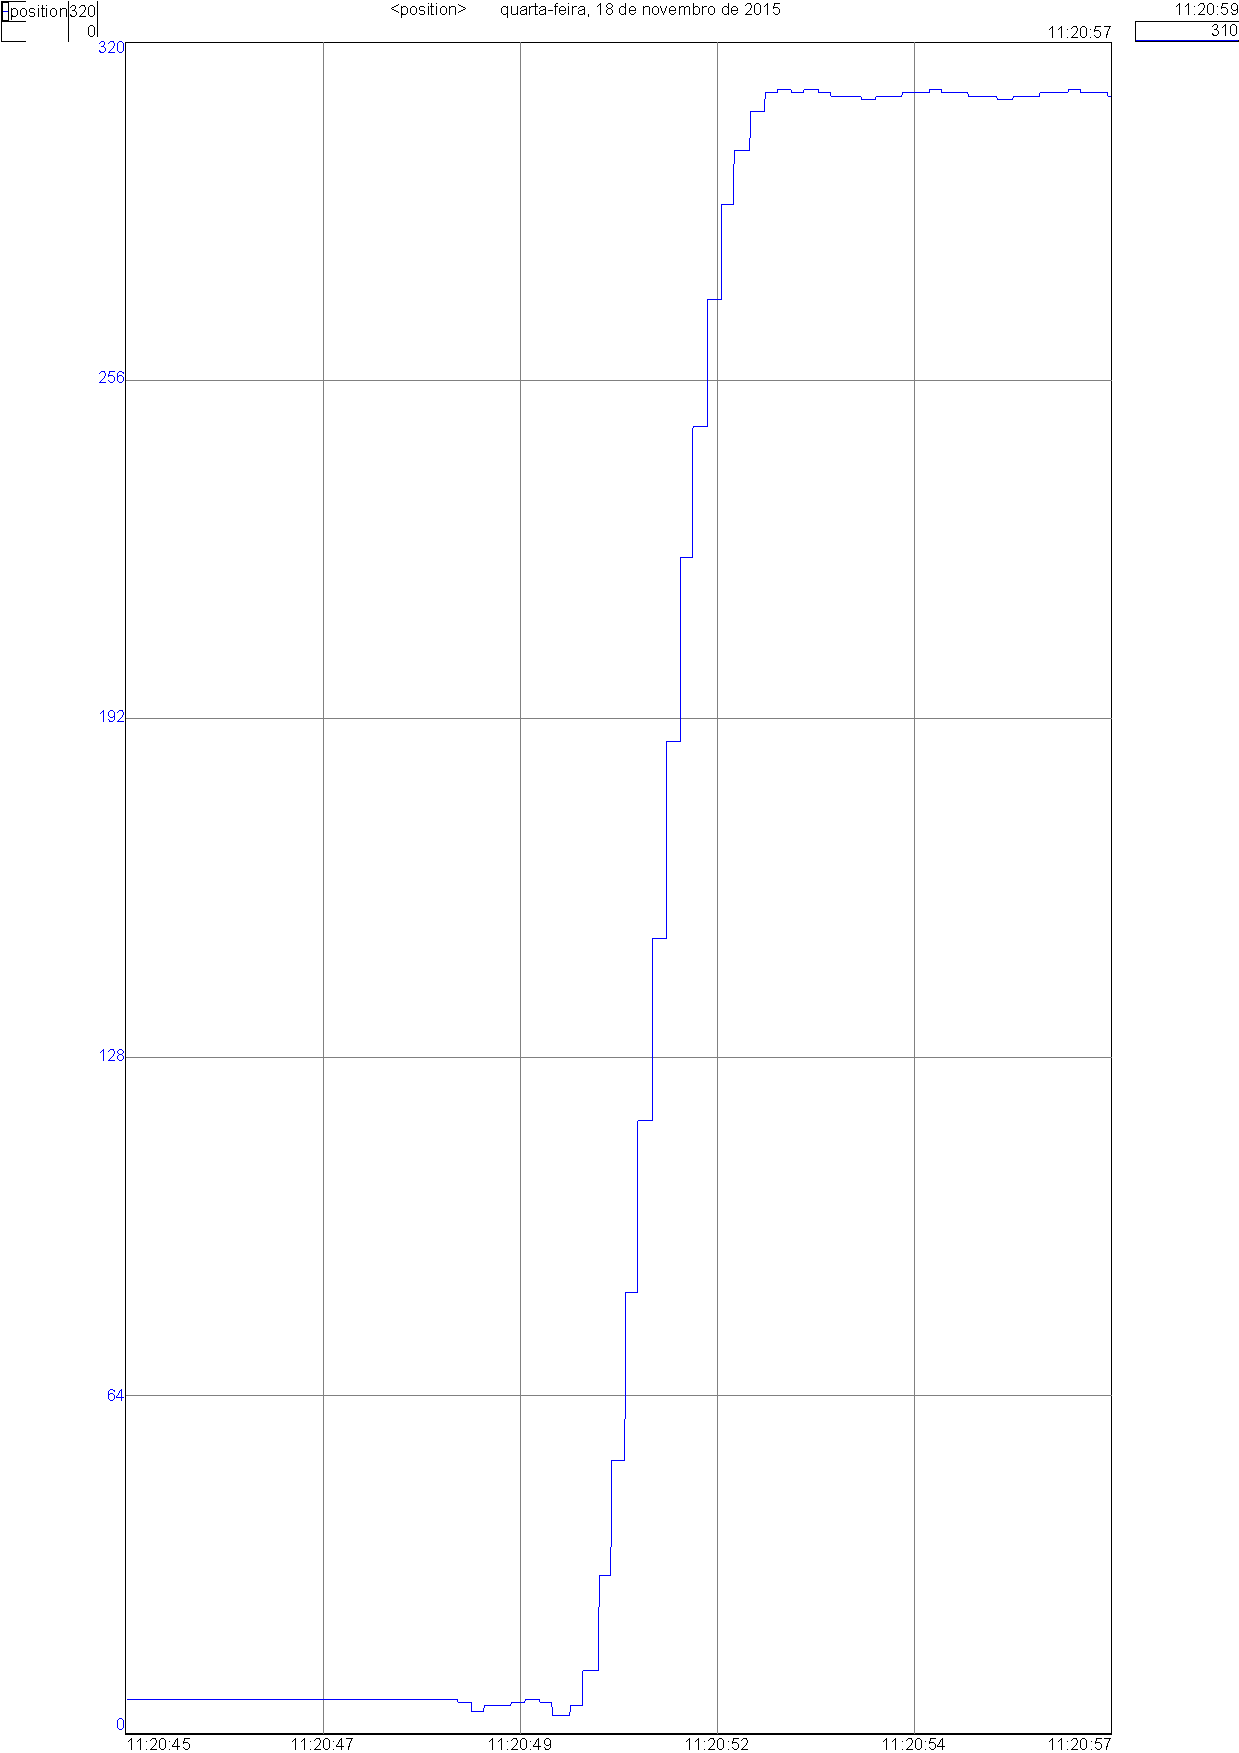
\includegraphics[width=1\linewidth,height=6cm]{figs/resultados/malha_aberta_1/trajetoriaObtidaModelada.pdf}
        \caption{Resultado com Velocidade Modelada para Excursão de 30cm}
        \label{trajetoriaObtidaModelada}
    \end{minipage}%
    \hspace{0.1cm}
    \begin{minipage}{0.45\textwidth}
        \centering
        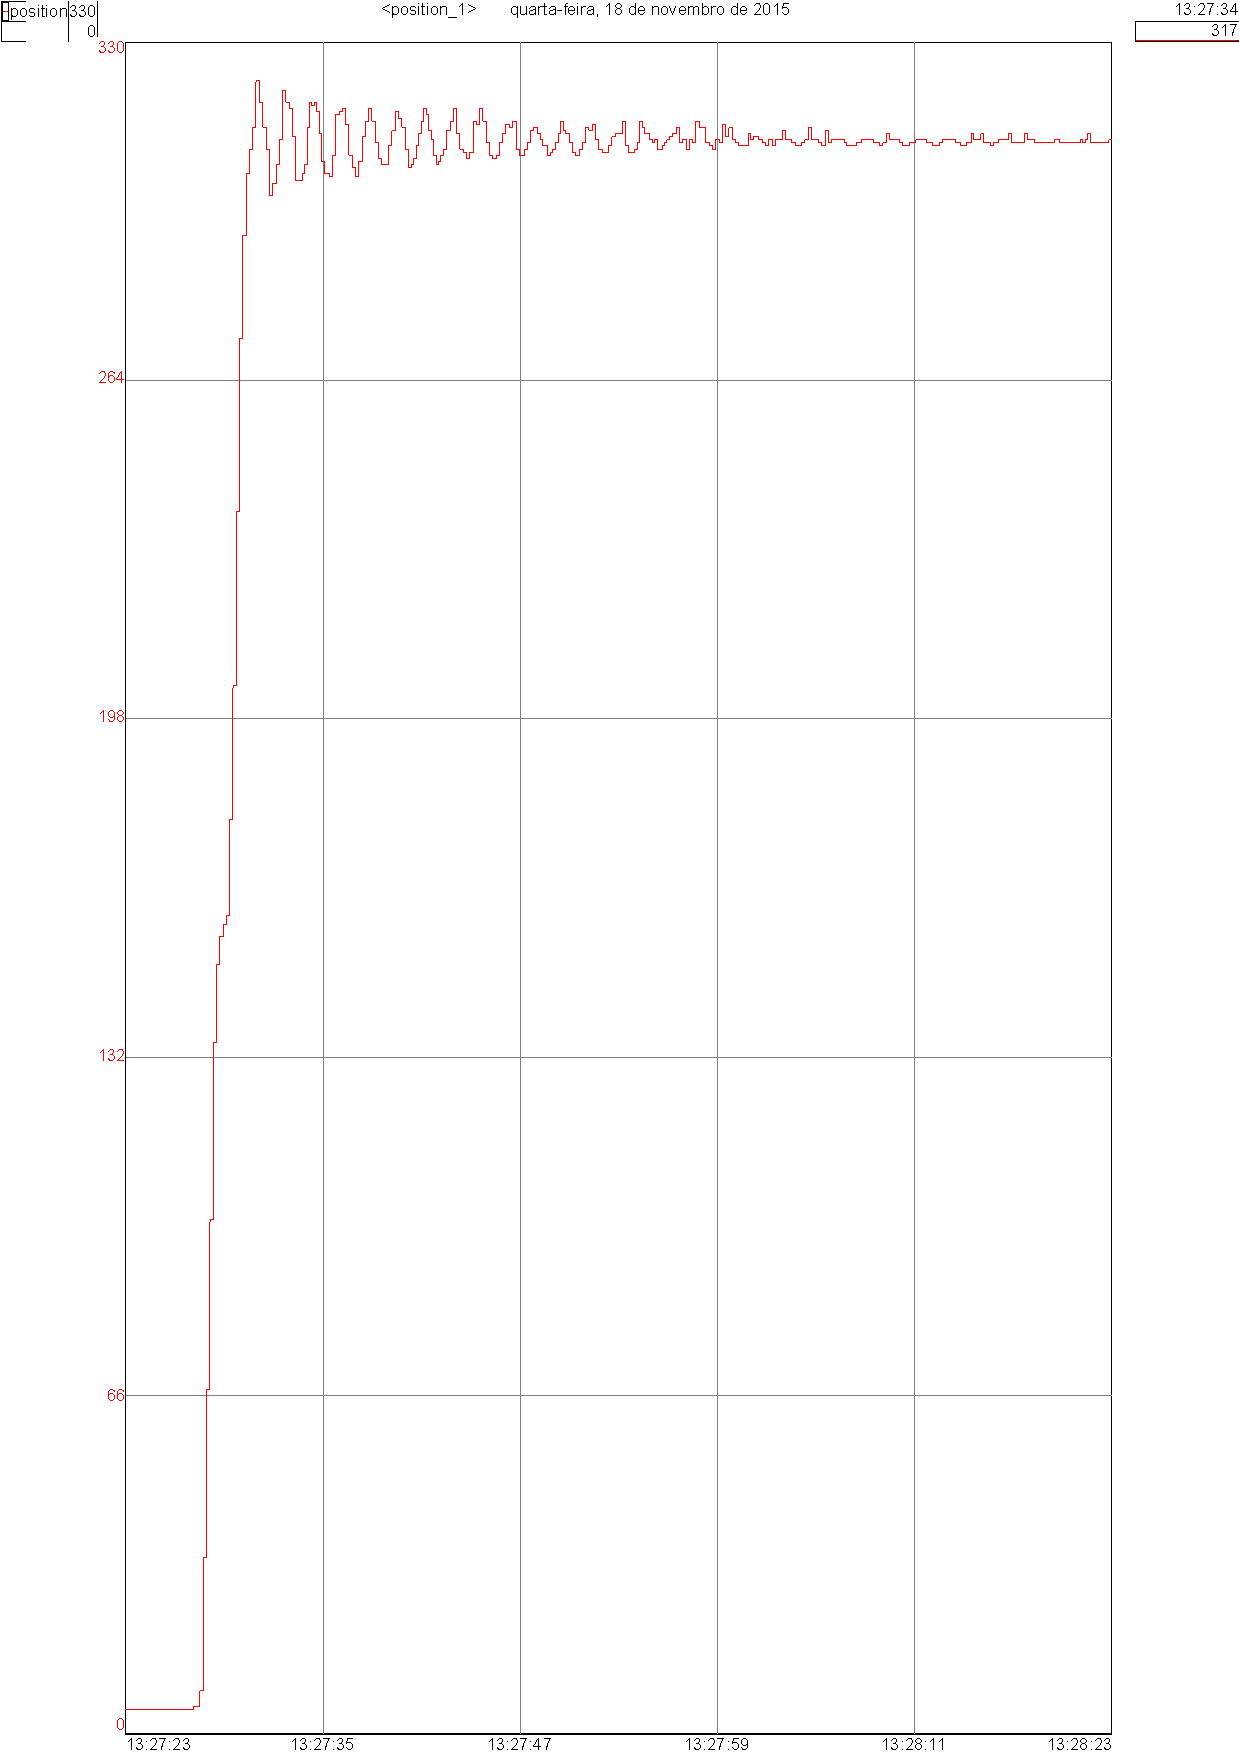
\includegraphics[width=1\linewidth,height=6cm]{figs/resultados/malha_aberta_1/trajetoriaObtidaVConstante.pdf}
        \caption{Resultado com Velocidade Constante para Excursão de 30cm}
        \label{trajetoriaObtidaVConstante}
    \end{minipage}
\end{figure}

\subsection{Excursão de 20cm}
Na prática, o diâmetro do \textit{riser} e de sua massa é bem menor que o comprimento do mesmo. Daí, é importante testar uma menor excursão. Além disso, esse teste terá menor tempo de movimentação e resultará numa velocidade média maior que o caso anterior. Desta forma, maiores oscilações são esperadas e o controle se torna mais difícil.

A trajetória de posição obtida é apresentada na Figura \ref{DeslocamentoT2} e a sua derivada é apresentada na Figura \ref{VelocidadeT2}. O período da tarefa eventual foi escolhido em $100\mathrm{ms}$. O resultado experimental\footnote{Controle Malha Aberta Modelado, 20cm - \url{https://youtu.be/wg1Wq_6VRSg}. Acesso em 29/11/2015.} apresentou mais oscilações que o caso anterior, mas está bem controlado, conforme se vê na Figura \ref{percurso20cmBom}. O resultado com velocidade constante\footnote{Controle Malha Aberta a Velocidade Constante, 20cm - \url{https://youtu.be/Ges2-eYy69k}. Acesso em 29/11/2015.} está na Figura \ref{percurso20cmRuim} e nota-se que o resultado ficou bem pior. A velocidade média foi cerca de $\overline{v} \approx \frac{200\mathrm{mm}}{1.5\mathrm{s}} = 133.3\mathrm{mm}/\mathrm{s}$. %TODO verificar se a velocidade de 133.3mm foi de fato utilizada no programa

\begin{figure}[!htb]
    \centering
    \begin{minipage}{.45\textwidth}
        \centering
        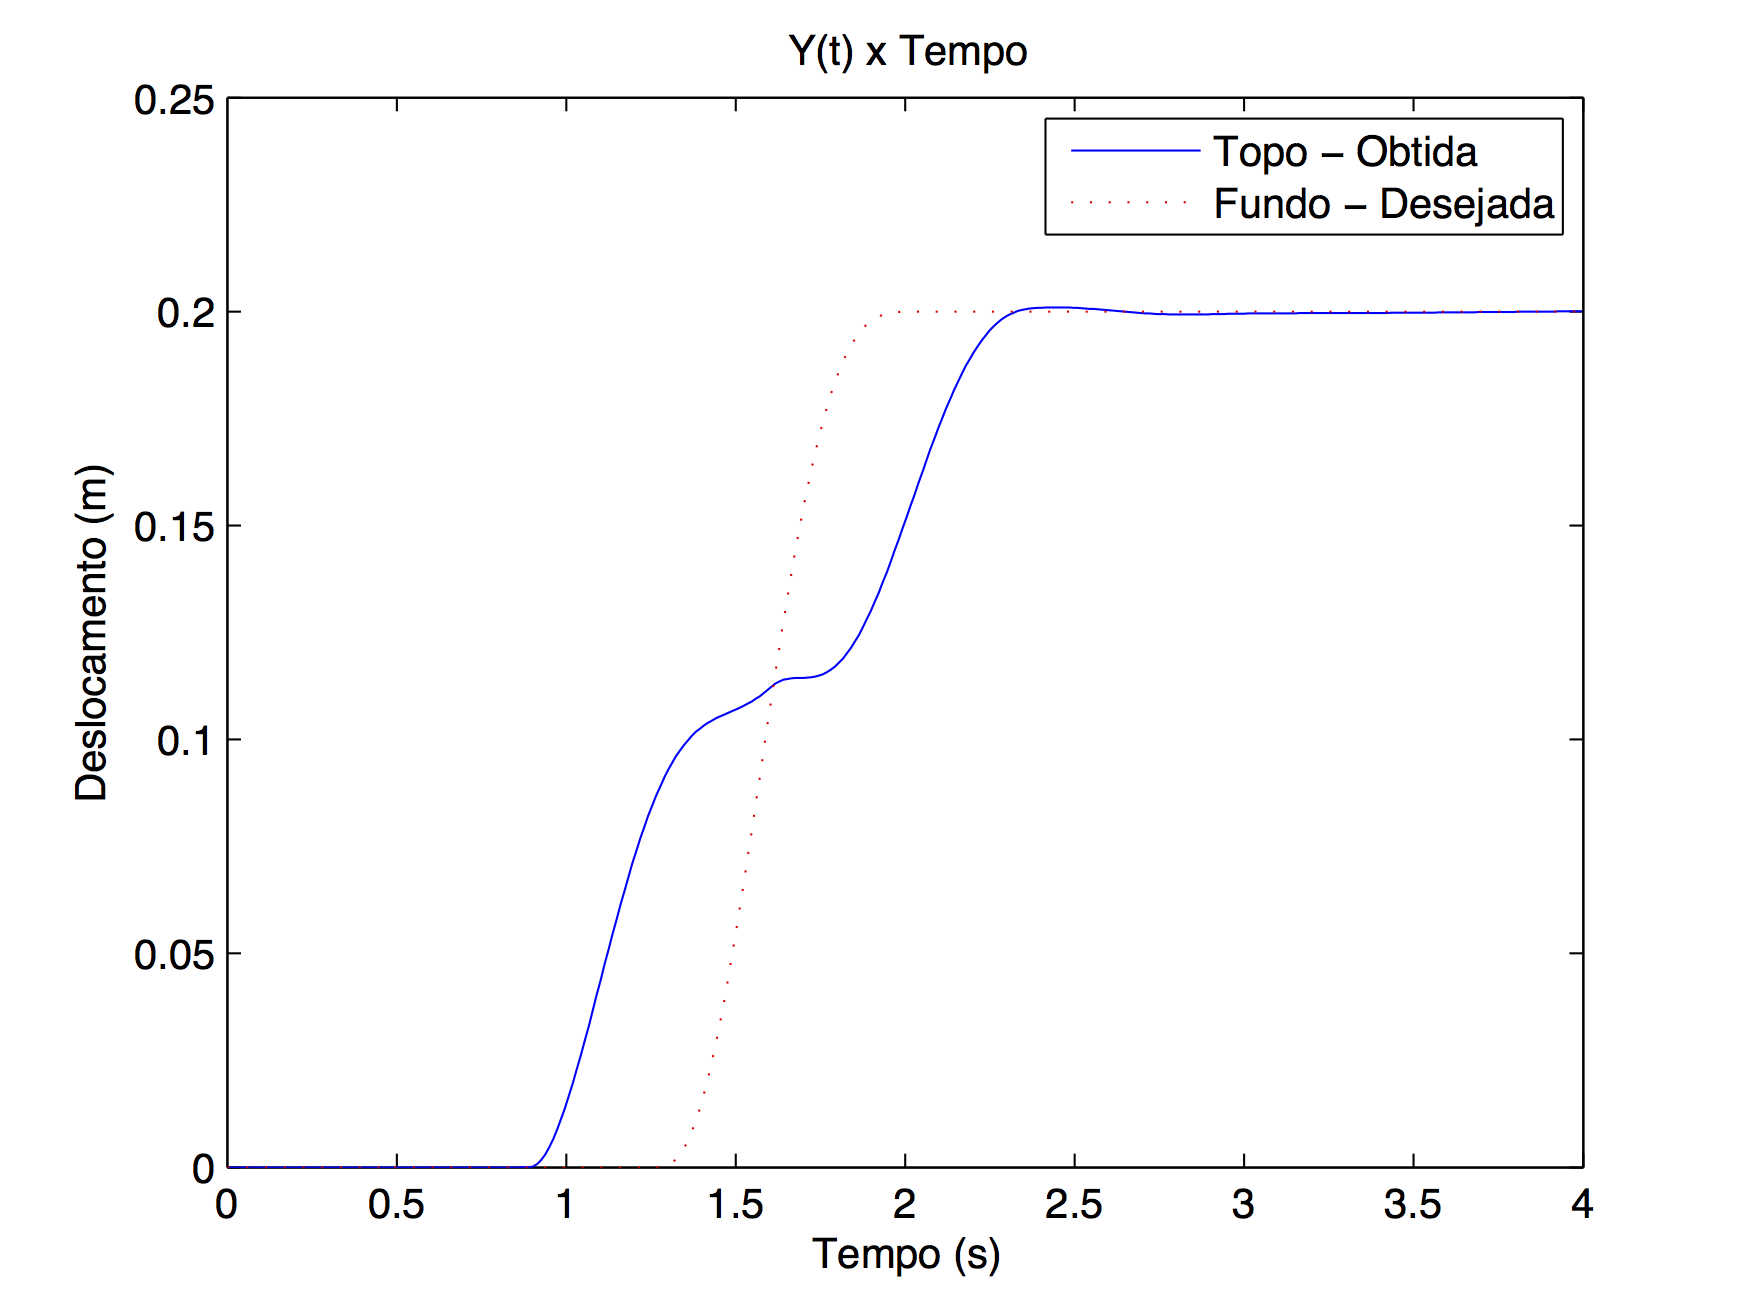
\includegraphics[width=1\linewidth]{figs/resultados/malha_aberta_2/DeslocamentoT2}
        \caption{Referência de Posição para Excursão de 20cm}
        \label{DeslocamentoT2}
    \end{minipage}%
    \hspace{0.1cm}
    \begin{minipage}{0.45\textwidth}
        \centering
        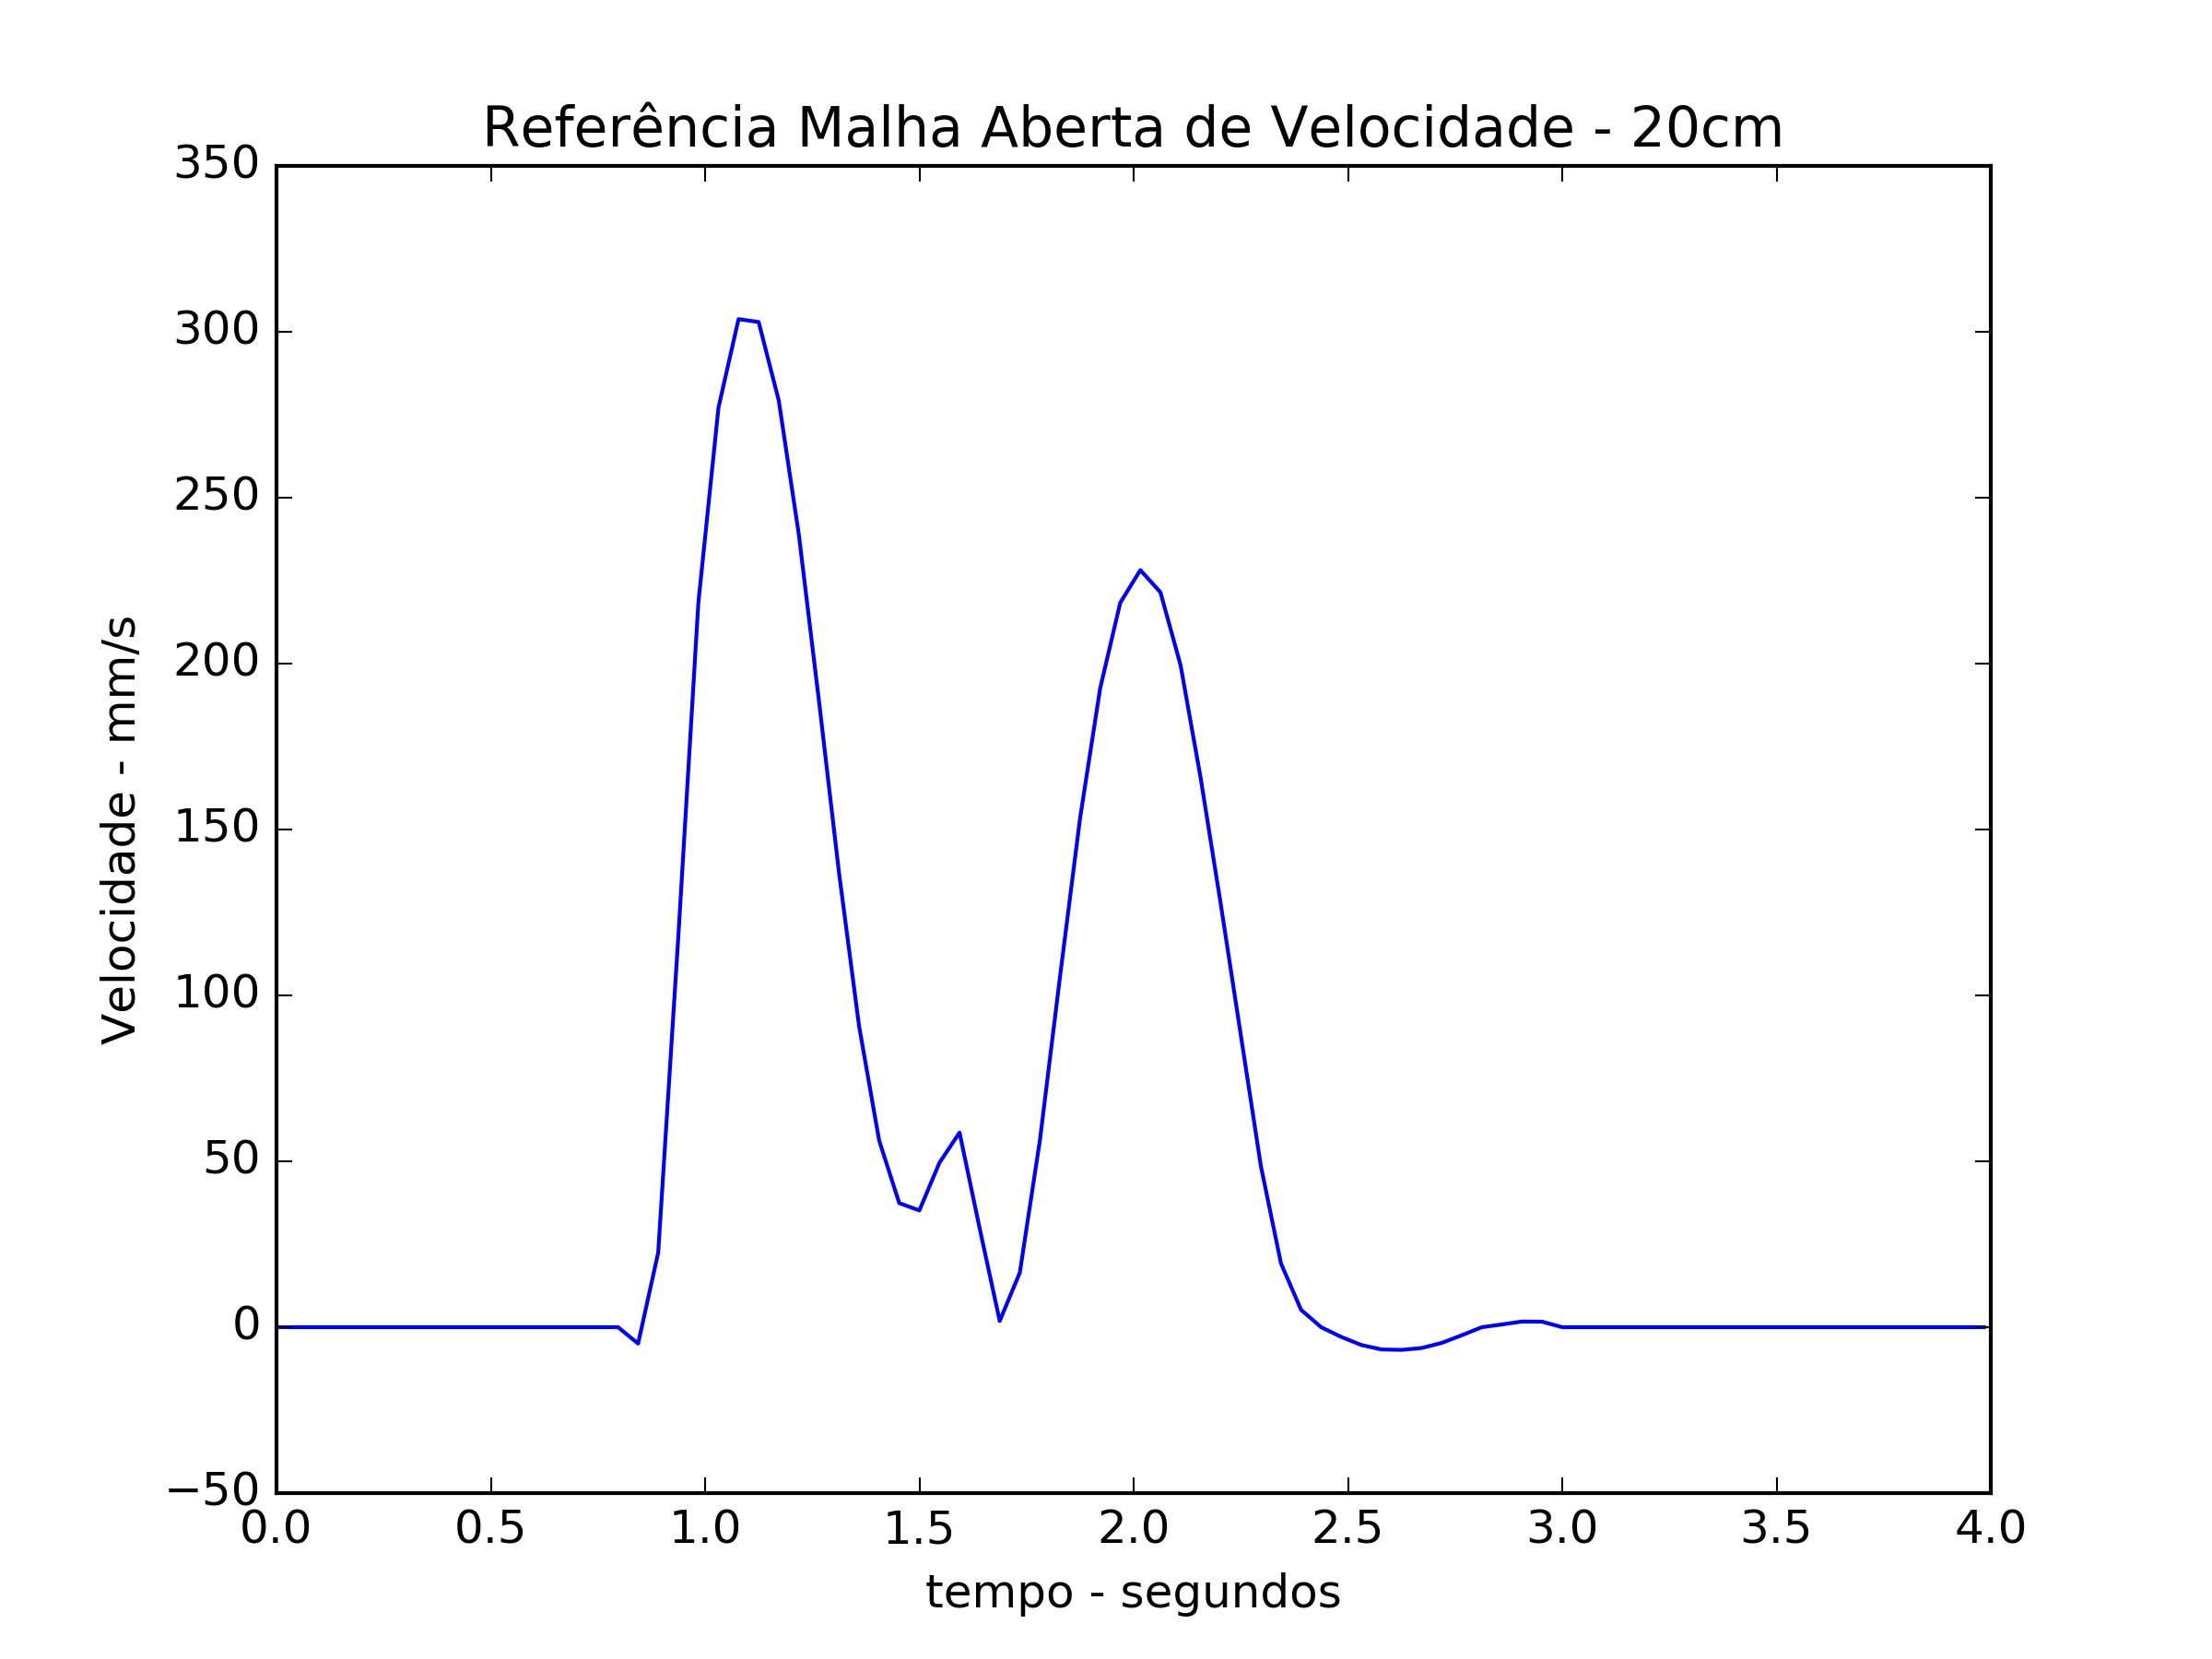
\includegraphics[width=1\linewidth]{figs/resultados/malha_aberta_2/VelocidadeT2}
        \caption{Referência de Velocidade para Excursão de 20cm}
        \label{VelocidadeT2}
    \end{minipage}
\end{figure}

\begin{figure}[!htb]
    \centering
    \begin{minipage}{.45\textwidth}
        \centering
        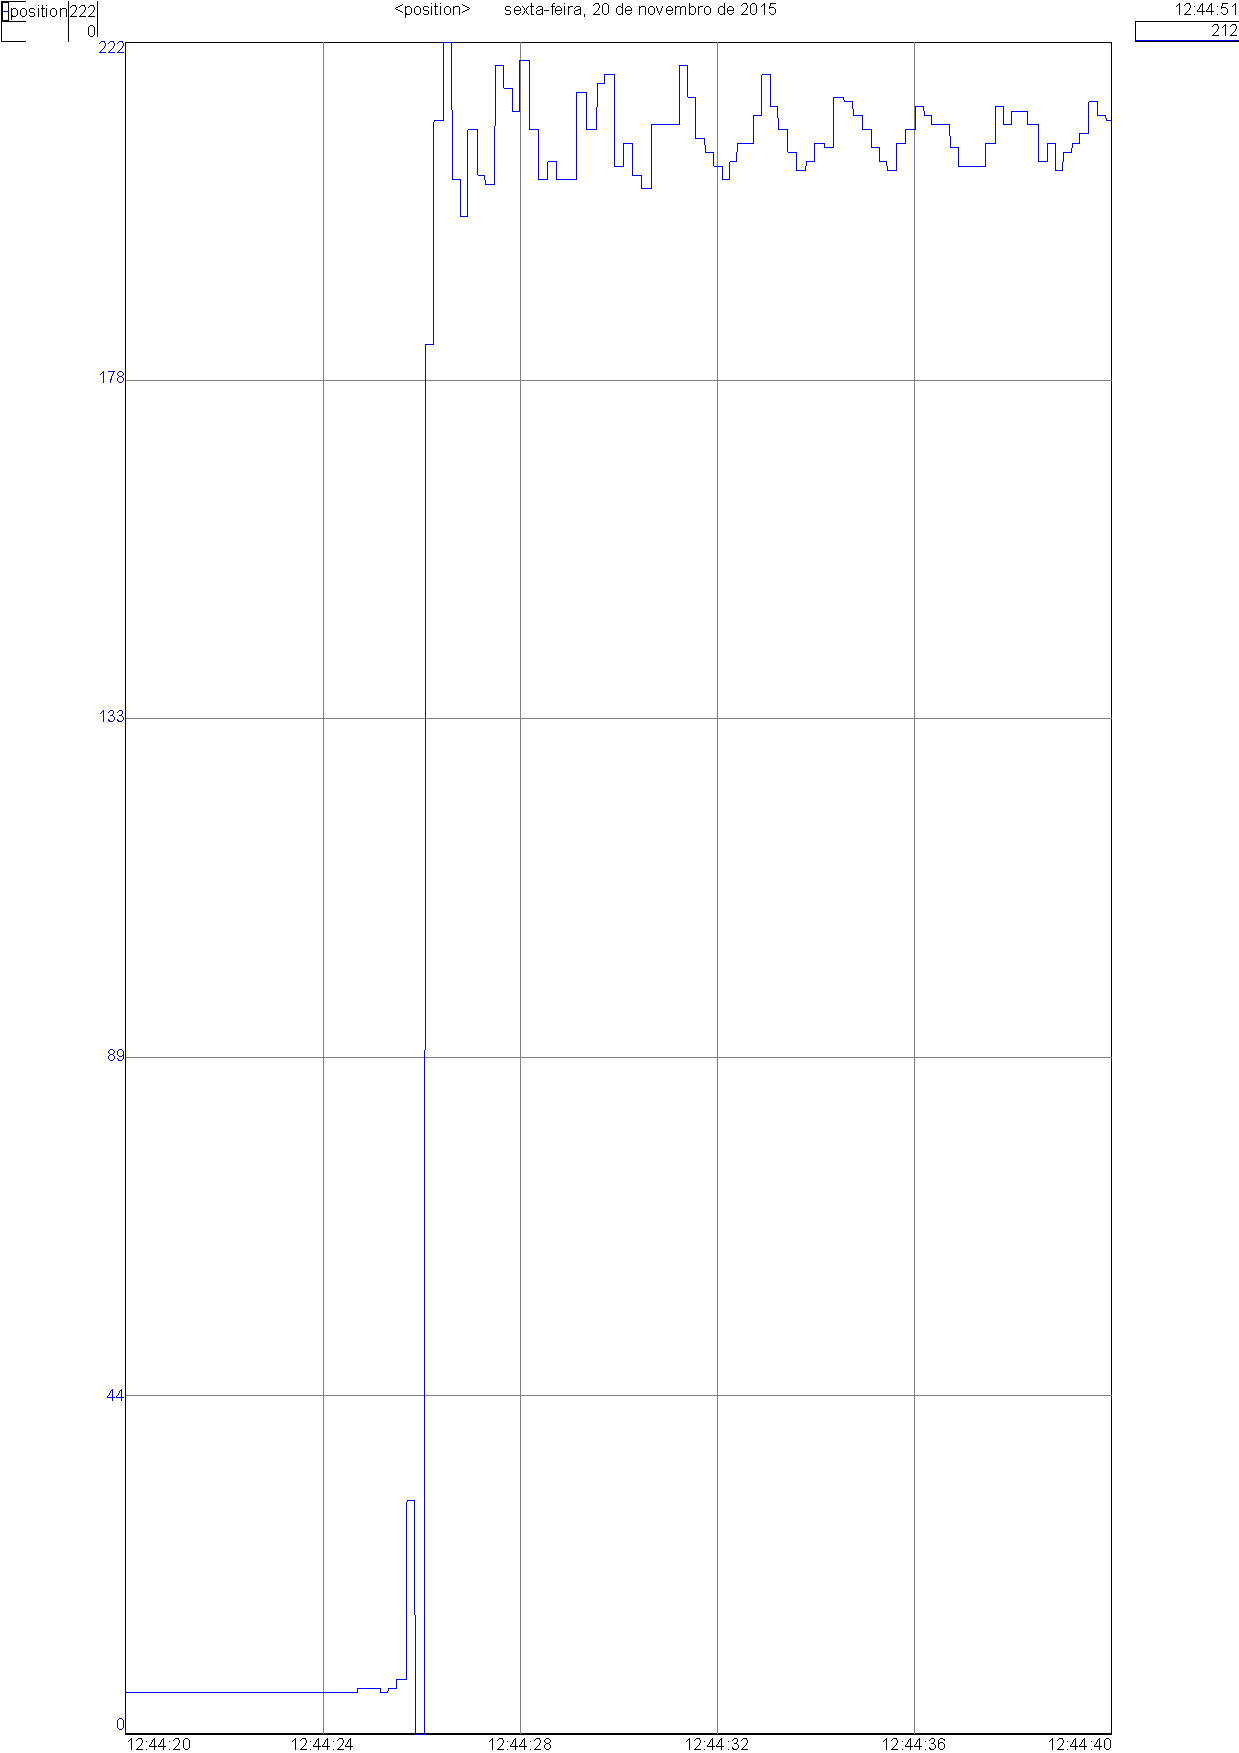
\includegraphics[width=1\linewidth,height=6cm]{figs/resultados/malha_aberta_2/percurso20cmBom.pdf}
        \caption{Resultado com Velocidade Modelada para Excursão de 20cm}
        \label{percurso20cmBom}
    \end{minipage}%
    \hspace{0.1cm}
    \begin{minipage}{0.45\textwidth}
        \centering
        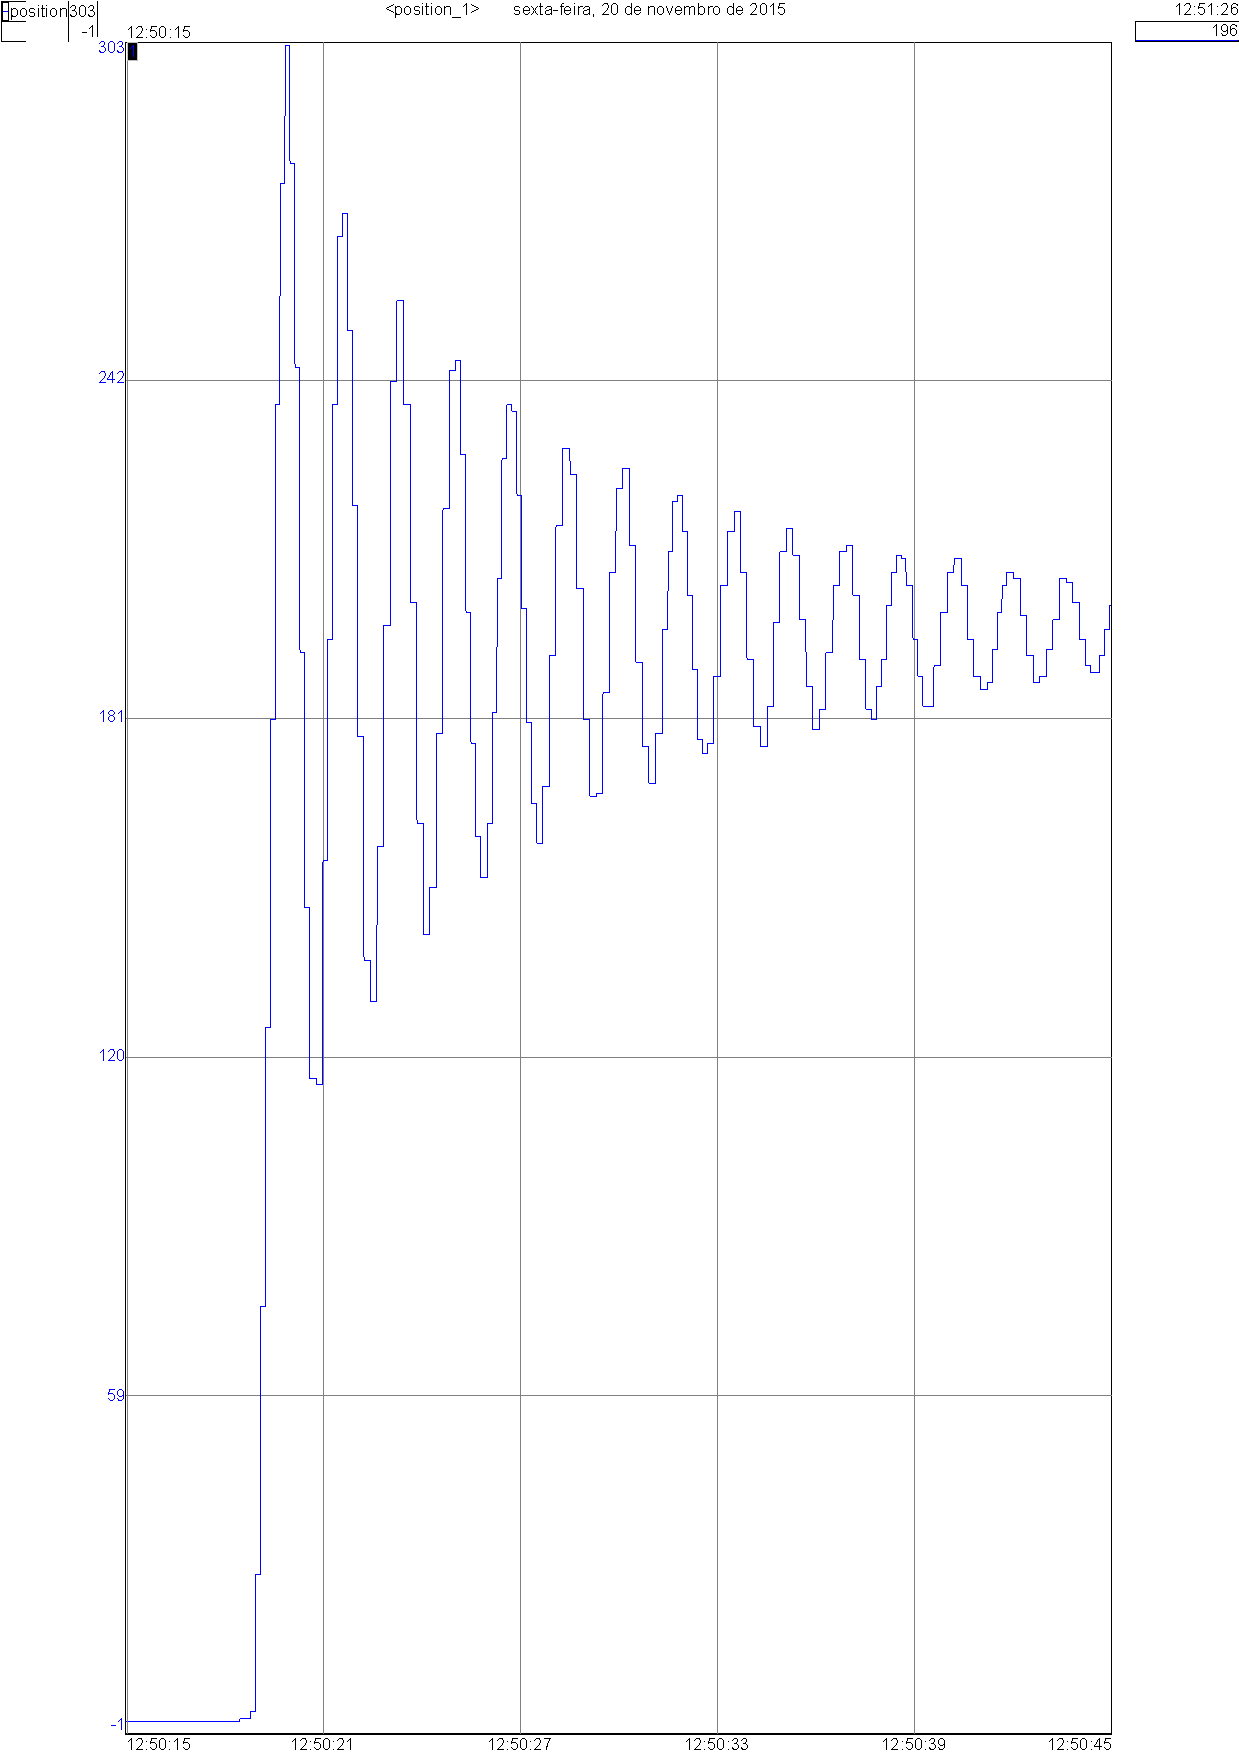
\includegraphics[width=1\linewidth,height=6cm]{figs/resultados/malha_aberta_2/percurso20cmRuim.pdf}
        \caption{Resultado com Velocidade Constante para Excursão de 20cm}
        \label{percurso20cmRuim}
    \end{minipage}
\end{figure}






\section{Malha fechada\label{malhafechadaSection}}
O controle em malha fechada deve ser capaz de compensar por perturbações, pois o sensor identifica o resultado da atuação e realimenta a informação no sistema. Neste trabalho, conseguiu-se configurar a câmera adequadamente e faz-se um teste em malha fechada de um controlador bem simples: um controlador proporcional.

\subsection{Controlador P}

O controlador proporcional utilizado tem o esquema conforme Figura \ref{mfechadaP}. A referência de posição $r = r(t)$ é a entrada do sistema e a saída medida pela câmera, $y_m$, é subtraída da referência para resultar no erro $e$, cuja unidade é dada em milímetros. A entrada da planta, $v$, é dad em $[\mathrm{u}/\mathrm{s}]$, conforme discutido anteriormente na subseção \ref{calibracaoServomotorSecao}. Desta forma, a unidade de $K_p$ é $\left[\frac{\mathrm{u}}{\mathrm{mm}\cdot\mathrm{s}}\right]$.

\begin{figure}[!ht]
\centering
\begin{tikzpicture}[auto, node distance=2cm,>=latex']
% We start by placing the blocks
\node [input, name=input] {};
\node [sum, right of=input] (sum) {};
\node [block, right of=sum] (controller) {$K_p$};
\node [block, right of=controller, pin={[pinstyle]above:Perturbações},
node distance=3cm] (system) {Planta};
% We draw an edge between the controller and system block to 
% calculate the coordinate u. We need it to place the measurement block. 
\draw [->] (controller) -- node[name=u] {$v$} (system);
\node [output, right of=system] (output) {};
\node [block, below of=u] (measurements) {Câmera};

% Once the nodes are placed, connecting them is easy. 
\draw [draw,->] (input) -- node {$r$} (sum);
\draw [->] (sum) -- node {$e$} (controller);
\draw [->] (system) -- node [name=y] {$y$}(output);
\draw [->] (y) |- (measurements);
\draw [->] (measurements) -| node[pos=0.99] {$-$} 
node [near end] {$y_m$} (sum);
\end{tikzpicture}
\caption{Malha fechada de controle\label{mfechadaP}}
\end{figure}

Valores de $K_p$ foram escolhidos empiricamente e o resultado para $K_p = 0.0025$\footnote{Controle Malha Fechada com Kp = 0.0025 - \url{https://youtu.be/mmT1ZwFBJ4s}. Acesso em 29/11/2015.} está na Figura \ref{MFProporcionalKpbaixo} enquanto para $K_p = 0.0050$\footnote{Controle Malha Fechada com Kp = 0.0050 - \url{https://youtu.be/sHh3yvBrek4}. Acesso em 29/11/2015.} está na Figura \ref{MFProporcionalKpmedio}.


\begin{figure}[!htb]
    \centering
    \begin{minipage}{.45\textwidth}
        \centering
        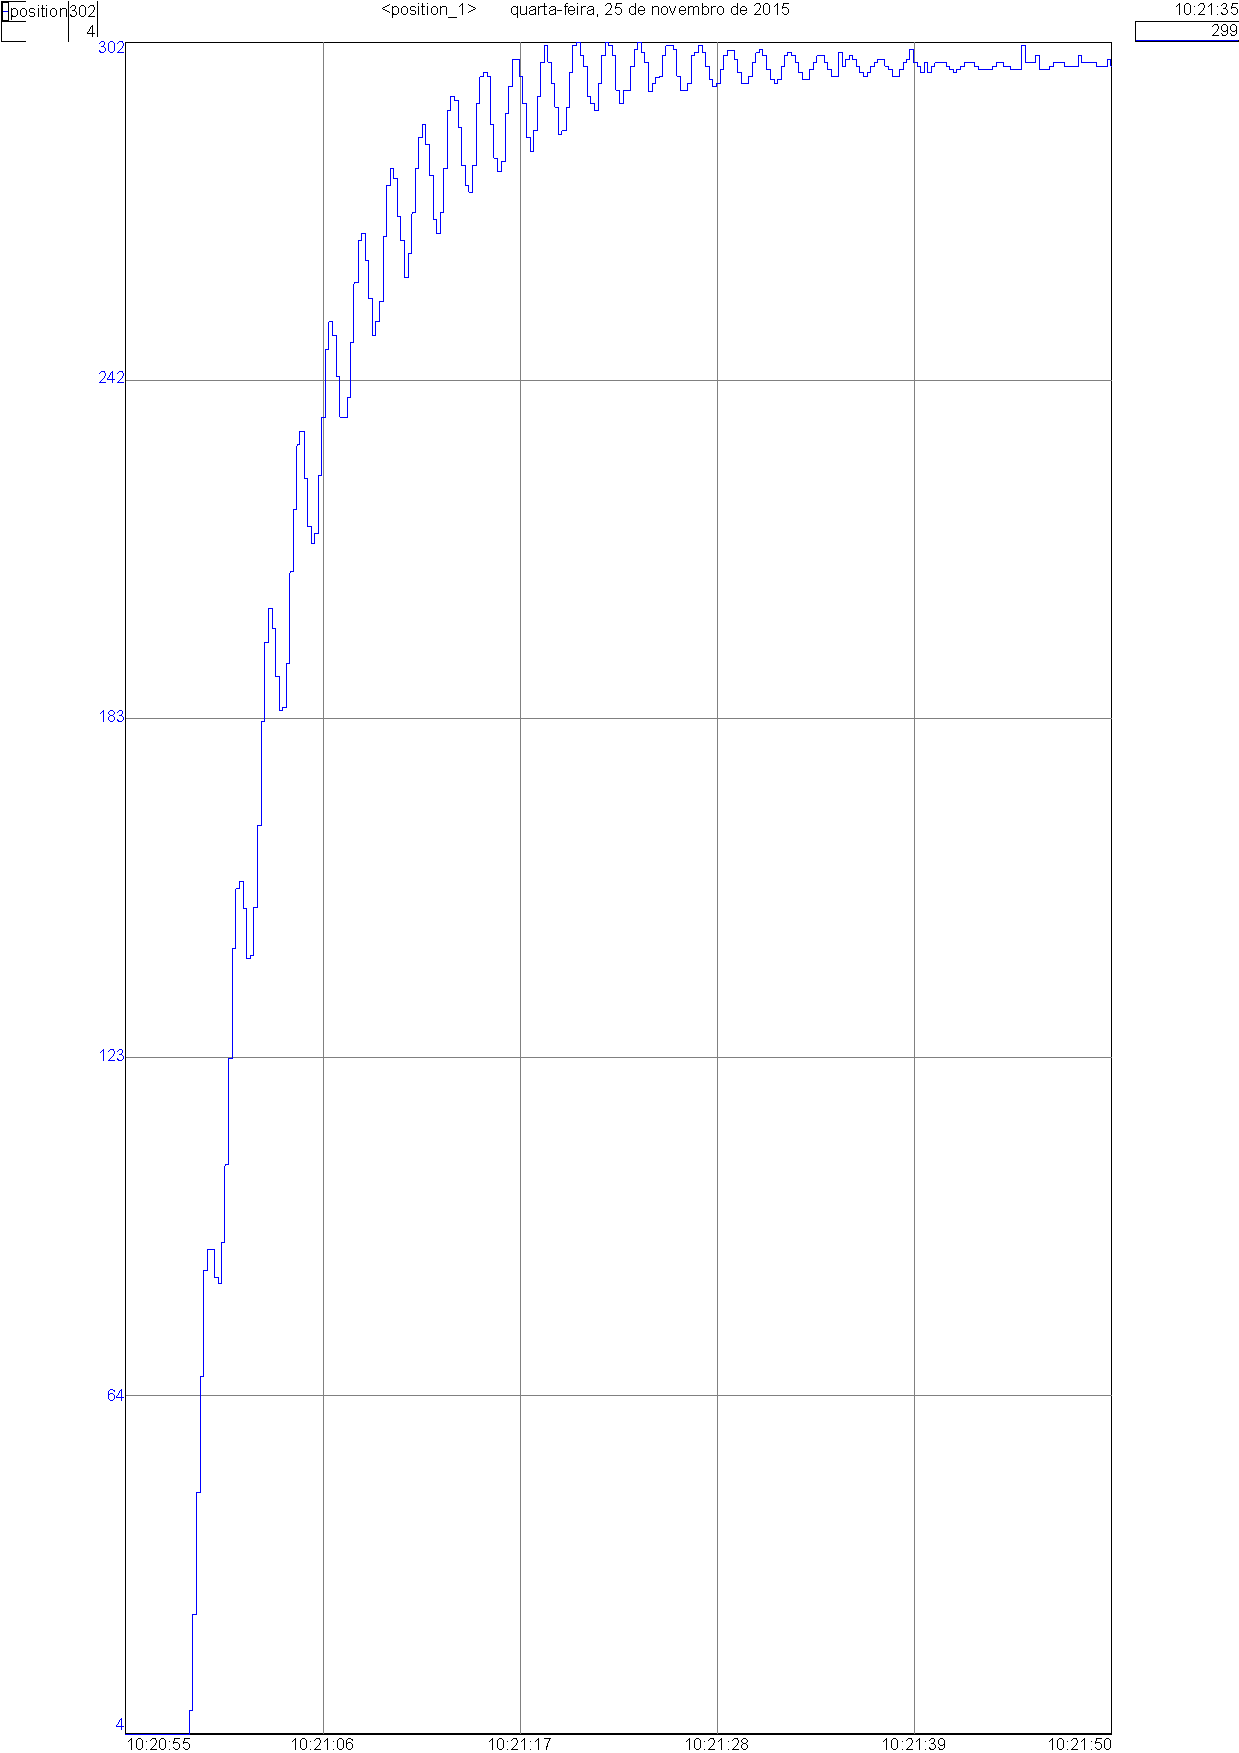
\includegraphics[width=1\linewidth,height=6cm]{figs/resultados/malha_fechada_P/MF_Proporcional_Kp_00025.pdf}
        \caption{Resultado com Malha Fechada Proporcional e $K_p = 0.0025\frac{\mathrm{u}}{\mathrm{mm}\cdot\mathrm{s}}$}
        \label{MFProporcionalKpbaixo}
    \end{minipage}%
    \hspace{0.1cm}
    \begin{minipage}{0.45\textwidth}
        \centering
        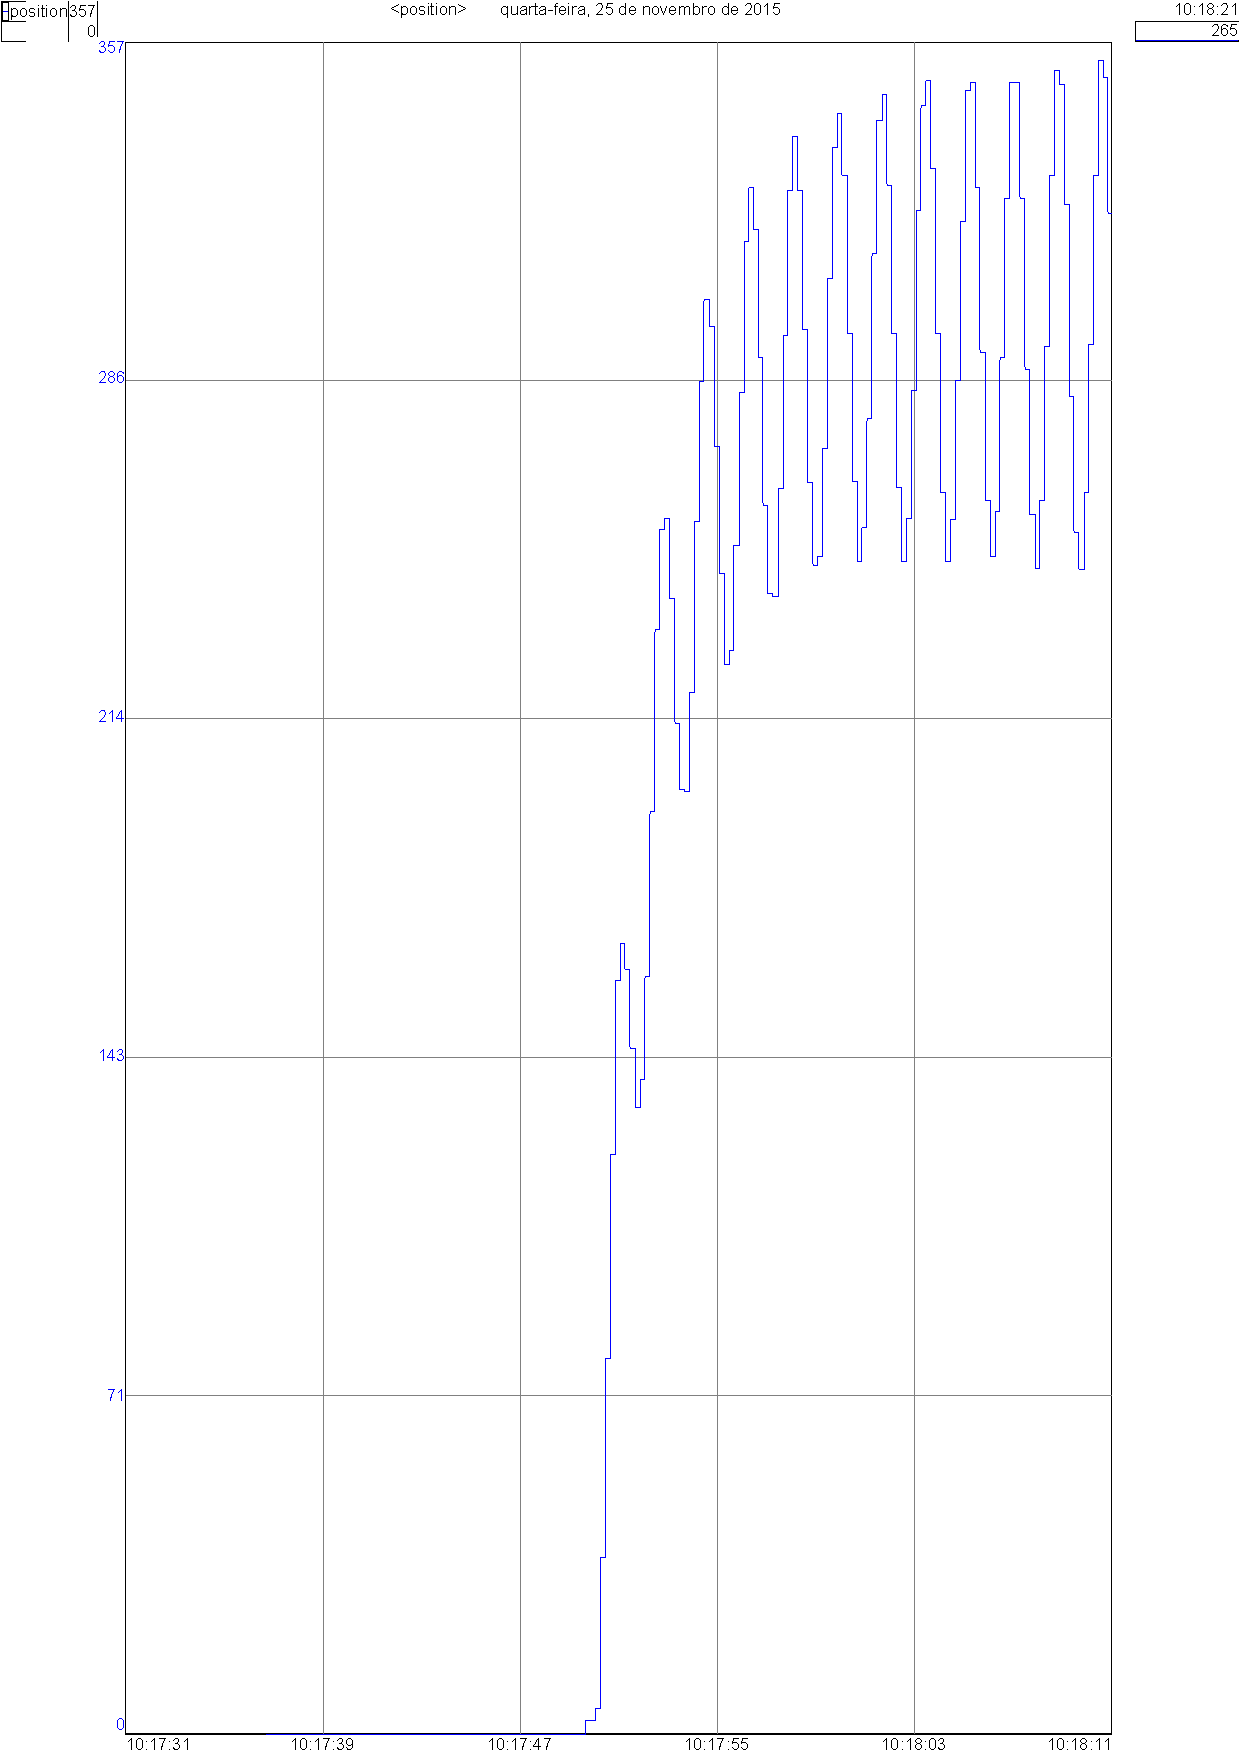
\includegraphics[width=1\linewidth,height=6cm]{figs/resultados/malha_fechada_P/MF_Proporcional_Kp_00050.pdf}
        \caption{Resultado com Malha Fechada Proporcional e $K_p = 0.0050\frac{\mathrm{u}}{\mathrm{mm}\cdot\mathrm{s}}$
        \label{MFProporcionalKpmedio}}
    \end{minipage}
\end{figure}

O período de amostragem utilizado foi de $100\mathrm{ms}$ e o ar condicionado estava ligado nas duas situações apresentadas e nota-se que o primeiro resultado é bem melhor que o segundo, tendo menos oscilações. No entanto, este resultado está aquém do obtido em malha aberta.

